%\documentclass[11pt]{article}
\documentclass[preprint,number,sort&compress,twocolumn,3p]{elsstyarticle}
\DeclareMathAlphabet{\scr}{U}{rsfs}{m}{n}
\usepackage{latexsym}
\usepackage{epsfig}
\usepackage[mathscr]{eucal}
\usepackage{amsfonts}
\usepackage{amscd}
\usepackage{amsmath}
\usepackage{array}
\usepackage{amssymb}
\usepackage{colordvi}
\usepackage{enumerate}
\usepackage{graphicx}
\usepackage{booktabs}
\usepackage[footnotesize]{caption}
\usepackage{fancyhdr} 
\usepackage{pdfpages}
\usepackage{slashed}
\usepackage{tabularx}
\usepackage{longtable}
\usepackage{array}
\usepackage{hyperref}
%\usepackage[draft]{hyperref}
\usepackage{relsize}
\usepackage{color}
%\usepackage[merge,numbers,compress]{natbib}
\usepackage{rotating}
\usepackage{cleveref}
%\crefformat{footnote}{#2\footnotemark[#1]#3}

\hypersetup{
	colorlinks=true,        % false: boxed links; true: colored links
	linkcolor=blue,          % color of internal links
	citecolor=black,        % color of links to bibliography
	filecolor=red,      % color of file links
	urlcolor=cyan           % color of external links
}

\setlength{\evensidemargin}{0cm}
\setlength{\oddsidemargin}{0cm}
\setlength{\topmargin}{0.00cm}
\setlength{\textwidth}{16.0cm}
\setlength{\textheight}{24.00cm}
\setlength{\headheight}{0cm}
\setlength{\headsep}{0cm}
\setlength{\voffset}{0cm}
\setlength{\paperheight}{29cm} 

\definecolor{ourbrown}{RGB}{155,100,15}
\definecolor{ourcyan}{RGB}{20,165,165}
\definecolor{ourpurple}{RGB}{145,0,140}
\definecolor{darkorange}{RGB}{225,100,0}
\definecolor{darkgreen}{RGB}{0,170,0}
\definecolor{darkgray}{RGB}{80,80,80}

\setlength{\marginparwidth}{20mm}

%% ---------------------------------
%% | New commands                  |
%% ---------------------------------


\newcommand{\eq}[1]{\begin{equation} #1 \end{equation}}
\newcommand{\eqa}[1]{\begin{eqnarray} #1 \end{eqnarray}}

\newcommand{\newc}{\newcommand}
\newc{\EW}{electroweak\;}
\newc{\DM}{dark matter\;}
\newc{\SM}{standard model\;}
\newc{\KK}{Kaluza-Klein\;}
\newc{\ff}{fragmentation function\;}
\newc{\be}{\begin{equation}}
\newc{\ee}{\end{equation}}
\newc{\bi}{\begin{itemize}}
\newc{\ei}{\end{itemize}}
\newc{\benu}{\begin{enumerate}}
\newc{\eenu}{\end{enumerate}}
\newc{\bc}{\begin{center}}
\newc{\ec}{\end{center}}
\newc{\bfig}{\begin{figure}}
\newc{\efig}{\end{figure}}
\newc{\neutone}{\tilde{\chi}^0_1}
\newc{\sigmav}{\langle\sigma v \rangle}
\newc{\lamhs}{\lambda_{H\!S}}
\newc{\logJ}{\log (J_{40^\circ}/J_{40^\circ\!,\,\text{nom}})}
\newc{\sigJ}{\sigma_{\log\!J}}
\DeclareMathSymbol{\Gamma}{\mathalpha}{letters}{"00}
\DeclareMathSymbol{\Delta}{\mathalpha}{letters}{"01}
\DeclareMathSymbol{\Theta}{\mathalpha}{letters}{"02}
\DeclareMathSymbol{\Lambda}{\mathalpha}{letters}{"03}
\DeclareMathSymbol{\Xi}{\mathalpha}{letters}{"04}
\DeclareMathSymbol{\Pi}{\mathalpha}{letters}{"05}
\DeclareMathSymbol{\Sigma}{\mathalpha}{letters}{"06}
\DeclareMathSymbol{\Upsilon}{\mathalpha}{letters}{"07}
\DeclareMathSymbol{\Phi}{\mathalpha}{letters}{"08}
\DeclareMathSymbol{\Psi}{\mathalpha}{letters}{"09}
\DeclareMathSymbol{\Omega}{\mathalpha}{letters}{"0A}
\DeclareMathSymbol{\varGamma}{\mathalpha}{operators}{"00}
\DeclareMathSymbol{\varDelta}{\mathalpha}{operators}{"01}
\DeclareMathSymbol{\varTheta}{\mathalpha}{operators}{"02}
\DeclareMathSymbol{\varLambda}{\mathalpha}{operators}{"03}
\DeclareMathSymbol{\varXi}{\mathalpha}{operators}{"04}
\DeclareMathSymbol{\varPi}{\mathalpha}{operators}{"05}
\DeclareMathSymbol{\varSigma}{\mathalpha}{operators}{"06}
\DeclareMathSymbol{\varUpsilon}{\mathalpha}{operators}{"07}
\DeclareMathSymbol{\varPhi}{\mathalpha}{operators}{"08}
\DeclareMathSymbol{\varPsi}{\mathalpha}{operators}{"09}
\DeclareMathSymbol{\varOmega}{\mathalpha}{operators}{"0A}
\DeclareMathOperator{\sgn}{sgn}
\DeclareMathOperator\arctanh{arctanh}
\renewcommand{\vec}[1]{\boldsymbol{#1}}
\newcommand{\D}{\mathrm{d}}
\newcommand{\E}{\mathrm{e}}
\newcommand{\I}{{\rm i}}
\newcommand{\hn}{h^0}
\newcommand{\Hn}{{H^0}}
\newcommand{\An}{A^0}
\newcommand{\Hp}{{H^\pm}}
\newcommand{\Gn}{G^0}
\newcommand{\Gp}{G^\pm}
\newcommand{\lam}{\lambda}
\newcommand{\lamL}{\lambda_L}
\newcommand{\HO}{H^0}
\def\bea{\begin{eqnarray}}
\def\eea{\end{eqnarray}}
\newcommand{\stau}{{\widetilde{\tau}}}		
\newcommand{\stopo}{{\widetilde{t}}}
\newcommand{\sboto}{{\widetilde{b}}}		
\newcommand{\snutau}{{\widetilde{\nu}_\tau}}
\newcommand{\neu}{{\widetilde{\chi}^0}}
\newcommand{\mstau}{m_{\stau_1}} 
\newcommand{\mstop}{m_{\stopo_1}}
\newcommand{\msbot}{m_{\sboto_1}}
\newcommand{\msnutau}{m_{\snutau}}
\newcommand{\mstautwo}{m_{\stau_2}} 
\newcommand{\msle}{{m_{\s{l}}}}   
\newcommand{\mne}{{m_{\s{\chi}^0_1}}}
\newcommand{\mchar}{{m_{\s{\chi}^\pm_1}}}  
\newcommand{\msq}{{m_{\widetilde{q}}}}
\newcommand{\mgo}{{m_{\widetilde{g}}}}
\newcommand{\thest}{\theta_{\stau}}
\newcommand{\s}[1]{\widetilde{#1}}
\newcommand{\MEV}{\ensuremath{\,\textnormal{MeV}}}
\newcommand{\GEV}{\ensuremath{\,\textnormal{GeV}}}
\newcommand{\TEV}{\ensuremath{\,\textnormal{TeV}}}
\newcommand{\smo}{\textsc{SModelS}}

%\newcommand{\min}{\text{min}}
%\newcommand{\max}{\text{max}}

%%%%%%%%%%%%%%%%%%%%%%
% temporary defs for comment environment
% to be removed upon submission
\newcommand{\com}[1]{\emph{\color{red}[#1]}}  % Comments
\newcommand{\blrm}{\emph{\color{red}[}}		
\newcommand{\brrm}{\emph{\color{red}]}}	
%%%%%%%%%%%%%%%%%%%%%%


\begin{document}

\title{{%\bf
Constraining new physics with
searches for long-lived particles with SModelS}}

\date{August 15, 2018}
\author[a]{Jan Heisig}
\address[a]{Institute for Theoretical Particle Physics and Cosmology, RWTH Aachen University, 52056 Aachen, Germany}
\author[b]{Sabine Kraml}
\address[b]{Laboratoire de Physique Subatomique et de Cosmologie, Universit\'e
    Grenoble-Alpes, CNRS/IN2P3, 53 Avenue des Martyrs, F-38026 Grenoble, France}
\author[c]{Andre Lessa}
\address[c]{Centro de Ci\^encias Naturais e Humanas, Universidade Federal do ABC, Santo Andr\'e, 09210-580 SP, Brazil}


\begin{abstract}
Long-lived particles have received an increasingly attention from
both the experimental and theoretical communities, due to their possible connection
to Dark Matter and novel collider signatures.
In this letter we discuss how some of the collider results for long-lived particles
re-interpreted within simplified models can be a powerful tool for constraining interesting models. For this purpose we present an implementation of (lepton-like) heavy stable charge
particle (HSCP) and $R$-hadron signatures into \smo~1.2, including searches 
performed at the 8 and 13\,TeV LHC. Using the (publicly available) \smo~1.2
tool we investigate how these searches impact two physics scenarios:
the Two Higgs Inert Doublet Model (IDM) and a gravitino dark matter model containing long-lived staus. 
While missing energy searches are not able to constrain any significant
part of the cosmologically allowed parameter space of the IDM model,
we find that HSCP searches are sentive up to dark
matter masses of 580\,GeV (for small mass splittings within the inert
doublet). The gravitino dark matter model on the other hand can be constrained by both HSCP and $R$-hadron searches, which can become
valuable for determining the allowed ranges of the cosmological reheating temperature in this scenario.
\end{abstract}

\maketitle




%\thispagestyle{empty}
%\vfill
%\newpage
%\setcounter{page}{1}

%\tableofcontents

%===================================================================
\section{Introduction}\label{sec:intro}
%===================================================================


Exploring physics beyond the standard model (BSM) is one of the key scientific goals of 
the LHC\@.
% Investigating the implications of its (null-)results is an important step to answer
%the open questions of particle physics. 
Simplified models have turned out to provide useful 
benchmarks for interpreting LHC results and investigating their implications
aiming to answer the open questions of today's fundamental physics. \smo~\cite{Kraml:2013mwa,Ambrogi:2017neo}
provides a very efficient framework for this
reinterpretation by decomposing the signal of an arbitrary new physics model (respecting a  ${\cal{Z}}_2$ 
symmetry or a larger symmetry with a  ${\cal{Z}}==_2$ subgroup) into simplified model topologies.
This allows one to directly use the cross-section upper limits or efficiency maps provided by the experimental 
collaborations within the simplified model framework to constrain a larger
variety of BSM scenarios.\footnote{A certain degree of approximation is included in this procedure, since it  neglects properties like the exact production mechanism and the spin of the  particles in decays, see Ref.~\cite{Edelhauser:2014ena,Edelhauser:2015ksa,Arina:2015uea,Kraml:2016eti} for specific discussions.}

So far \smo~assumed that all stable particles were neutral and only included BSM searches for missing transverse momentum (MET).
However, it has widely been recognized that well-motivated
%to exploit the full LHC potential recently more exotic signatures have attracted
%growing interest.  
BSM theories can provide non-neutral long-lived particles (LLPs) leading to distinct signatures,
often providing great sensitivity at the LHC~\cite{}.
%\com{Motivations for LLPs? cite whitepaper?}
In this letter we make use of the novel features of \smo~1.2~\cite{smodlesnote} to investigate well-motivated
full BSM models containing LLPs.
Besides being able to decompose models with long-lived 
charged particles, this version also includes a treatment of metastable particles and constraints for heavy stable
charged particles (HSCPs) and $R$-hadrons\footnote{For simplicity we label electrically charged and color neutral heavy stable particles as HSCPs. Long-lived colored particles, which can hadronize and form electrically charged bound states are always referred to as $R$-hadrons.} in its database.
In particular, we improve upon previous work~\cite{Heisig:2015yla} adding 
efficiency maps for the CMS 13\,TeV HSCP analysis~\cite{CMS-PAS-EXO-16-036} and reconsidering the modeling of intermediate lifetimes.
We also include the experimental 
cross-section upper limits for the direct production of HSCPs~\cite{Khachatryan:2015lla,CMS-PAS-EXO-16-036} and $R$-hadrons~\cite{CMS-PAS-EXO-16-036}.
Finally, \smo~1.2 is made publicly available.\footnote{The SModelS tool and database are available at \href{http://smodels.hephy.at}{http://smodels.hephy.at}}

%\com{mention first paper, how SMS used for LLPs; tell what's the difference: 
%plublic available, better treatment finite lifetimes (justification), 13\,TeV results, $R$-hadron}

We make use of \smo~1.2 to investigate how the searches for HSCPs and $R$-hadrons mentioned above impact two new physics scenarios. 
The first one, the Two Higgs Inert Doublet Model (IDM), provides one of the simplest dark matter models supplementing the Standard Model by just one additional $SU(2)$ (Higgs) doublet. 
While MET searches are scarcely sensitive to the cosmologically allowed region of the IDM parameter space, 
we show that for small mass splittings within the inert doublet a large range of dark matter masses
can be tested by the HSCP searches.

Secondly, we consider the minimal supersymmetric standard model (MSSM) 
where the gravitino is assumed to be the lightest supersymmetric particle (LSP) and the stau to be next-to-LSP (NLSP). This is a cosmologically attractive scenario allowing to alleviate the gravitino problem~\cite{Weinberg:1982zq,Ellis:1984eq,Falomkin:1984eu,Ellis:1984er} and to accommodate large reheating temperatures $T_\text{R}\sim10^9\,$GeV
in the early Universe while respecting bounds from big bang nucleosynthesis (BBN)~\cite{}.
The complexity of the model reveals a large number of contributing topologies including
$R$-hadron signatures relevant for both squarks and gluinos when their decays are 3- or 4-body suppressed.
We show that the LLP results have the potential to be competitive with cosmological constraints and impact the allowed range for the reheating temperature.
\com{Some more refs?}

%\com{Introduce physics cases: IDM hard to constrain, very small mass splitting, sensitivity 
%regard finite lifetimes; Gravtino LSP, LL stau, several topologies incl. $R$-hadrons, much further than just direct production,.
%}

The remainder of this letter is structured as follows. In Sec.~\ref{sec:impl} we briefly
review the implementation of LLP signatures into \smo. The impact for the 
IDM and gravitino scenarios is presented in Sec.~\ref{sec:physapp}. 
We conclude in Sec.~\ref{sec:summary}.
%while in Secs.~\ref{sec:IDM} and~\ref{sec:grav}
%we apply \smo\ to the IDM and a gravitino dark matter scenario. We present out 
%conclusions in Sec.~\ref{sec:summary}. 
%In \ref{app:rec13} we detail the recasting of the HSCP analyses and validate the results.
%Finally, \ref{app:lifetime} provides a discussion of the weights for 
%intermediate lifetimes.
Finally, in \ref{app:rec13} and \ref{app:lifetime} we provide details about the recasting of the HSCP analyses 
and a discussion about the treatment of intermediate lifetimes, respectively.

%\com{To be introduced: HSCP, MET, LSP, NLSP, MSSM, pMSSM, LLP, IDM?}

%===================================================================
\section{Implementation in \smo}\label{sec:impl}
%===================================================================


Given the particle width, branching ratios (BRs) and total production cross-sections of a certain BSM model, \smo\ performs a decomposition of the input model into a coherent sum of simplified model 
topologies~\cite{Kraml:2013mwa,Ambrogi:2017neo}. 
Each topology represents a pair of (prompt) cascade decays which terminate
in a long-lived (BSM) particle. While previous versions 
assumed all particles to either have prompt decays or to be long-lived (in collider scales), version 1.2~\cite{smodlesnote} includes a calculation
for the fraction of prompt decays ($\mathcal{F}_\text{prompt}$) and decays outside the detector ($\mathcal{F}_\text{long}$), which
can be relevant for metastable particles with proper lifetimes within $\sim$few cm to $\sim$few m.~\cite{Heisig:2015yla}
These fractions are used during decomposition to 
rescale the branching ratios, thus resulting in an effective topology cross-section ($\tilde{\sigma}$) given by:
\begin{equation}
\label{eq:weights}
\tilde{\sigma} = \sigma_\text{prod}\left(\prod_i
\text{BR}_i \times \mathcal{F}_\text{prompt}^i \right)
\mathcal{F}_\text{long}^X \mathcal{F}_\text{long}^Y \,,
\end{equation}
where $\sigma_\text{prod}$ is the production cross-section of the mother particles and
$X,Y$ are the BSM final states of the two decay chains while $i$ runs over all intermediate 
BSM particles. Given the particle proper lifetime ($\tau$), the fraction of produced particles which decay promptly ($\mathcal{F}_\text{prompt}$)
and decay outside the detector ($\mathcal{F}_\text{prompt}$) can be approximated by:
\begin{equation}
\label{eq:fprompt}
\mathcal{F}_\text{prompt} = 1-\exp\left(-\frac{1}{c\tau}\left\langle\!\frac{\ell_\text{inner}}{\gamma \beta} \!\right\rangle_{\!\!\text{eff}\,}\right)
\end{equation}
and
\begin{equation}
\label{eq:Flong}
\mathcal{F}_\text{long} = \exp\left(-\frac{1}{c\tau}\left\langle\!\frac{\ell_\text{outer}}{\gamma \beta} \!\right\rangle_{\!\!\text{eff}\,}\right)\,,
\end{equation}
where we choose $\langle\ell_\text{inner}/\gamma\beta\rangle_\text{eff}=1\,$mm and $\langle\ell_\text{outer}/\gamma\beta\rangle_\text{eff}=7\,$m requiring long-lived particles to traverse the entire detector. A detailed motivation of the above expressions and values is given in~\ref{app:lifetime}. Note that this choice is conservative, since the signature of particles decaying inside the detector may provide additional sensitivity. However, such cases introduce a dependence on the decay products of the long-lived particle which is left for future work.

All topologies terminating in long-lived neutral particles provide a signature of missing transverse energy (MET) and can be constrained by  the bulk of SUSY searches. These, however, do not apply
to topologies which end with a color or electrically-charged BSM final state. In order to test these scenarios \smo~1.2 includes the CMS searches for HSCPs, color-octet (gluino-like) $R$-hadrons
and color-triplet (squark-like)  $R$-hadrons  at 8\,TeV~\cite{Chatrchyan:2013oca} and 13\,TeV~\cite{CMS-PAS-EXO-16-036} center-of-mass energies. For the 8\,TeV  HSCP results we make use of the recasting provided in Ref.~\cite{Khachatryan:2015lla}, while a dedicated recasting was performed for the 13\,TeV results (see~\ref{app:rec13} for details). This allowed us to compute efficiency maps for the 8 simplified model topologies introduced in Ref.~\cite{Heisig:2015yla}, which are included in the \smo~1.2 database.
For the $R$-hadron searches we consider only the direct production topology\footnote{As $R$-hadrons are strongly produced their production via cascade decays in typically expected to be less important.} and make use of the cross-section upper limits from Refs.~\cite{Chatrchyan:2013oca,CMS-PAS-EXO-16-036}, which are also included in the \smo\ database.

%
%Briefly review topologies used and our efficiency maps~\cite{Heisig:2015yla}.
%
%Refer to~\ref{app:rec13} for the recasting of the 13\,TeV analysis.
%
%
%Mention $R$-hadron searches.




%===================================================================
\section{Physics applications}\label{sec:physapp}
%===================================================================

In the following we use SModelS within two BSM scenarios and derive constraints 
on their parameter space. We consider the inert doubled model as well as a supersymmetric scenario with a gravitino LSP
and a stau NLSP\@.






%----------------------------------------------------------------------------------------------------------------
\subsection{The inert doublet model}\label{sec:IDM}
%----------------------------------------------------------------------------------------------------------------

%=======================
%    \                                           |
%      \                                         |
%        \                                       |
\begin{figure*}[h]
\centering
\setlength{\unitlength}{1\textwidth}
\begin{picture}(0.98,0.29)
\put(0.0,0.0){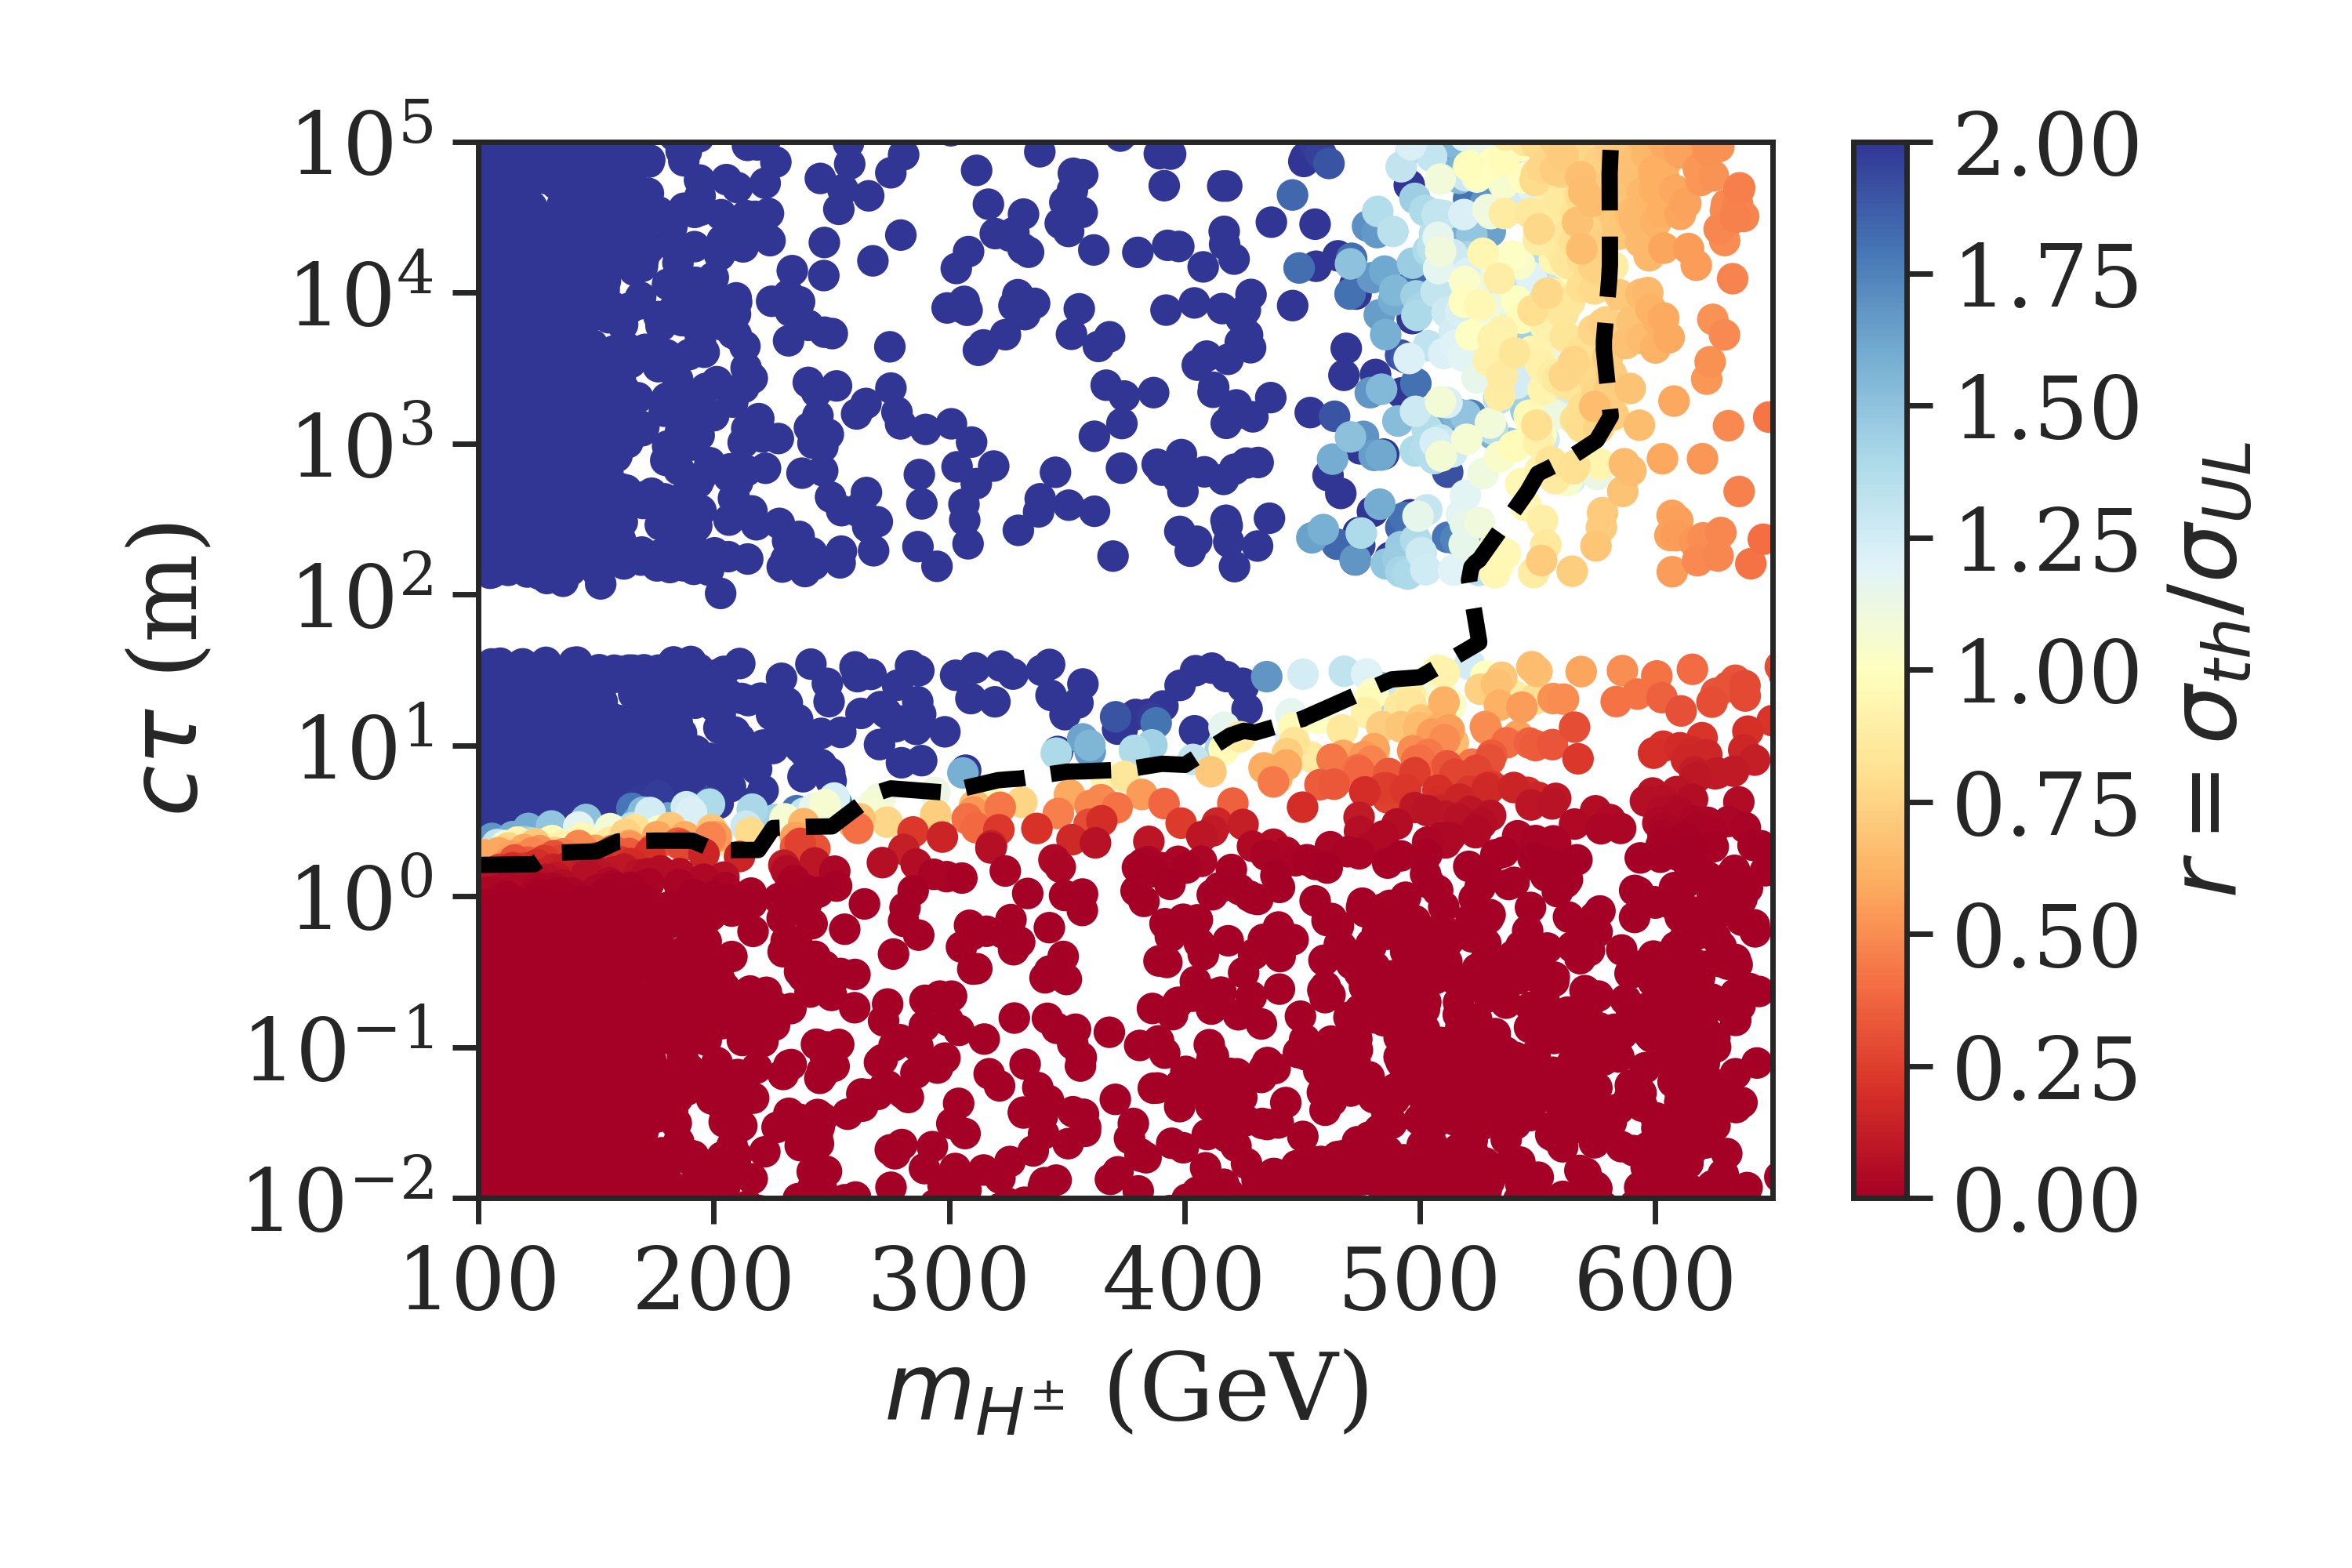
\includegraphics[clip, trim={0cm 0.6cm 0cm 0cm}, width=0.48\textwidth]{figures/IDM_points_r.png}}
\put(0.5,0.0){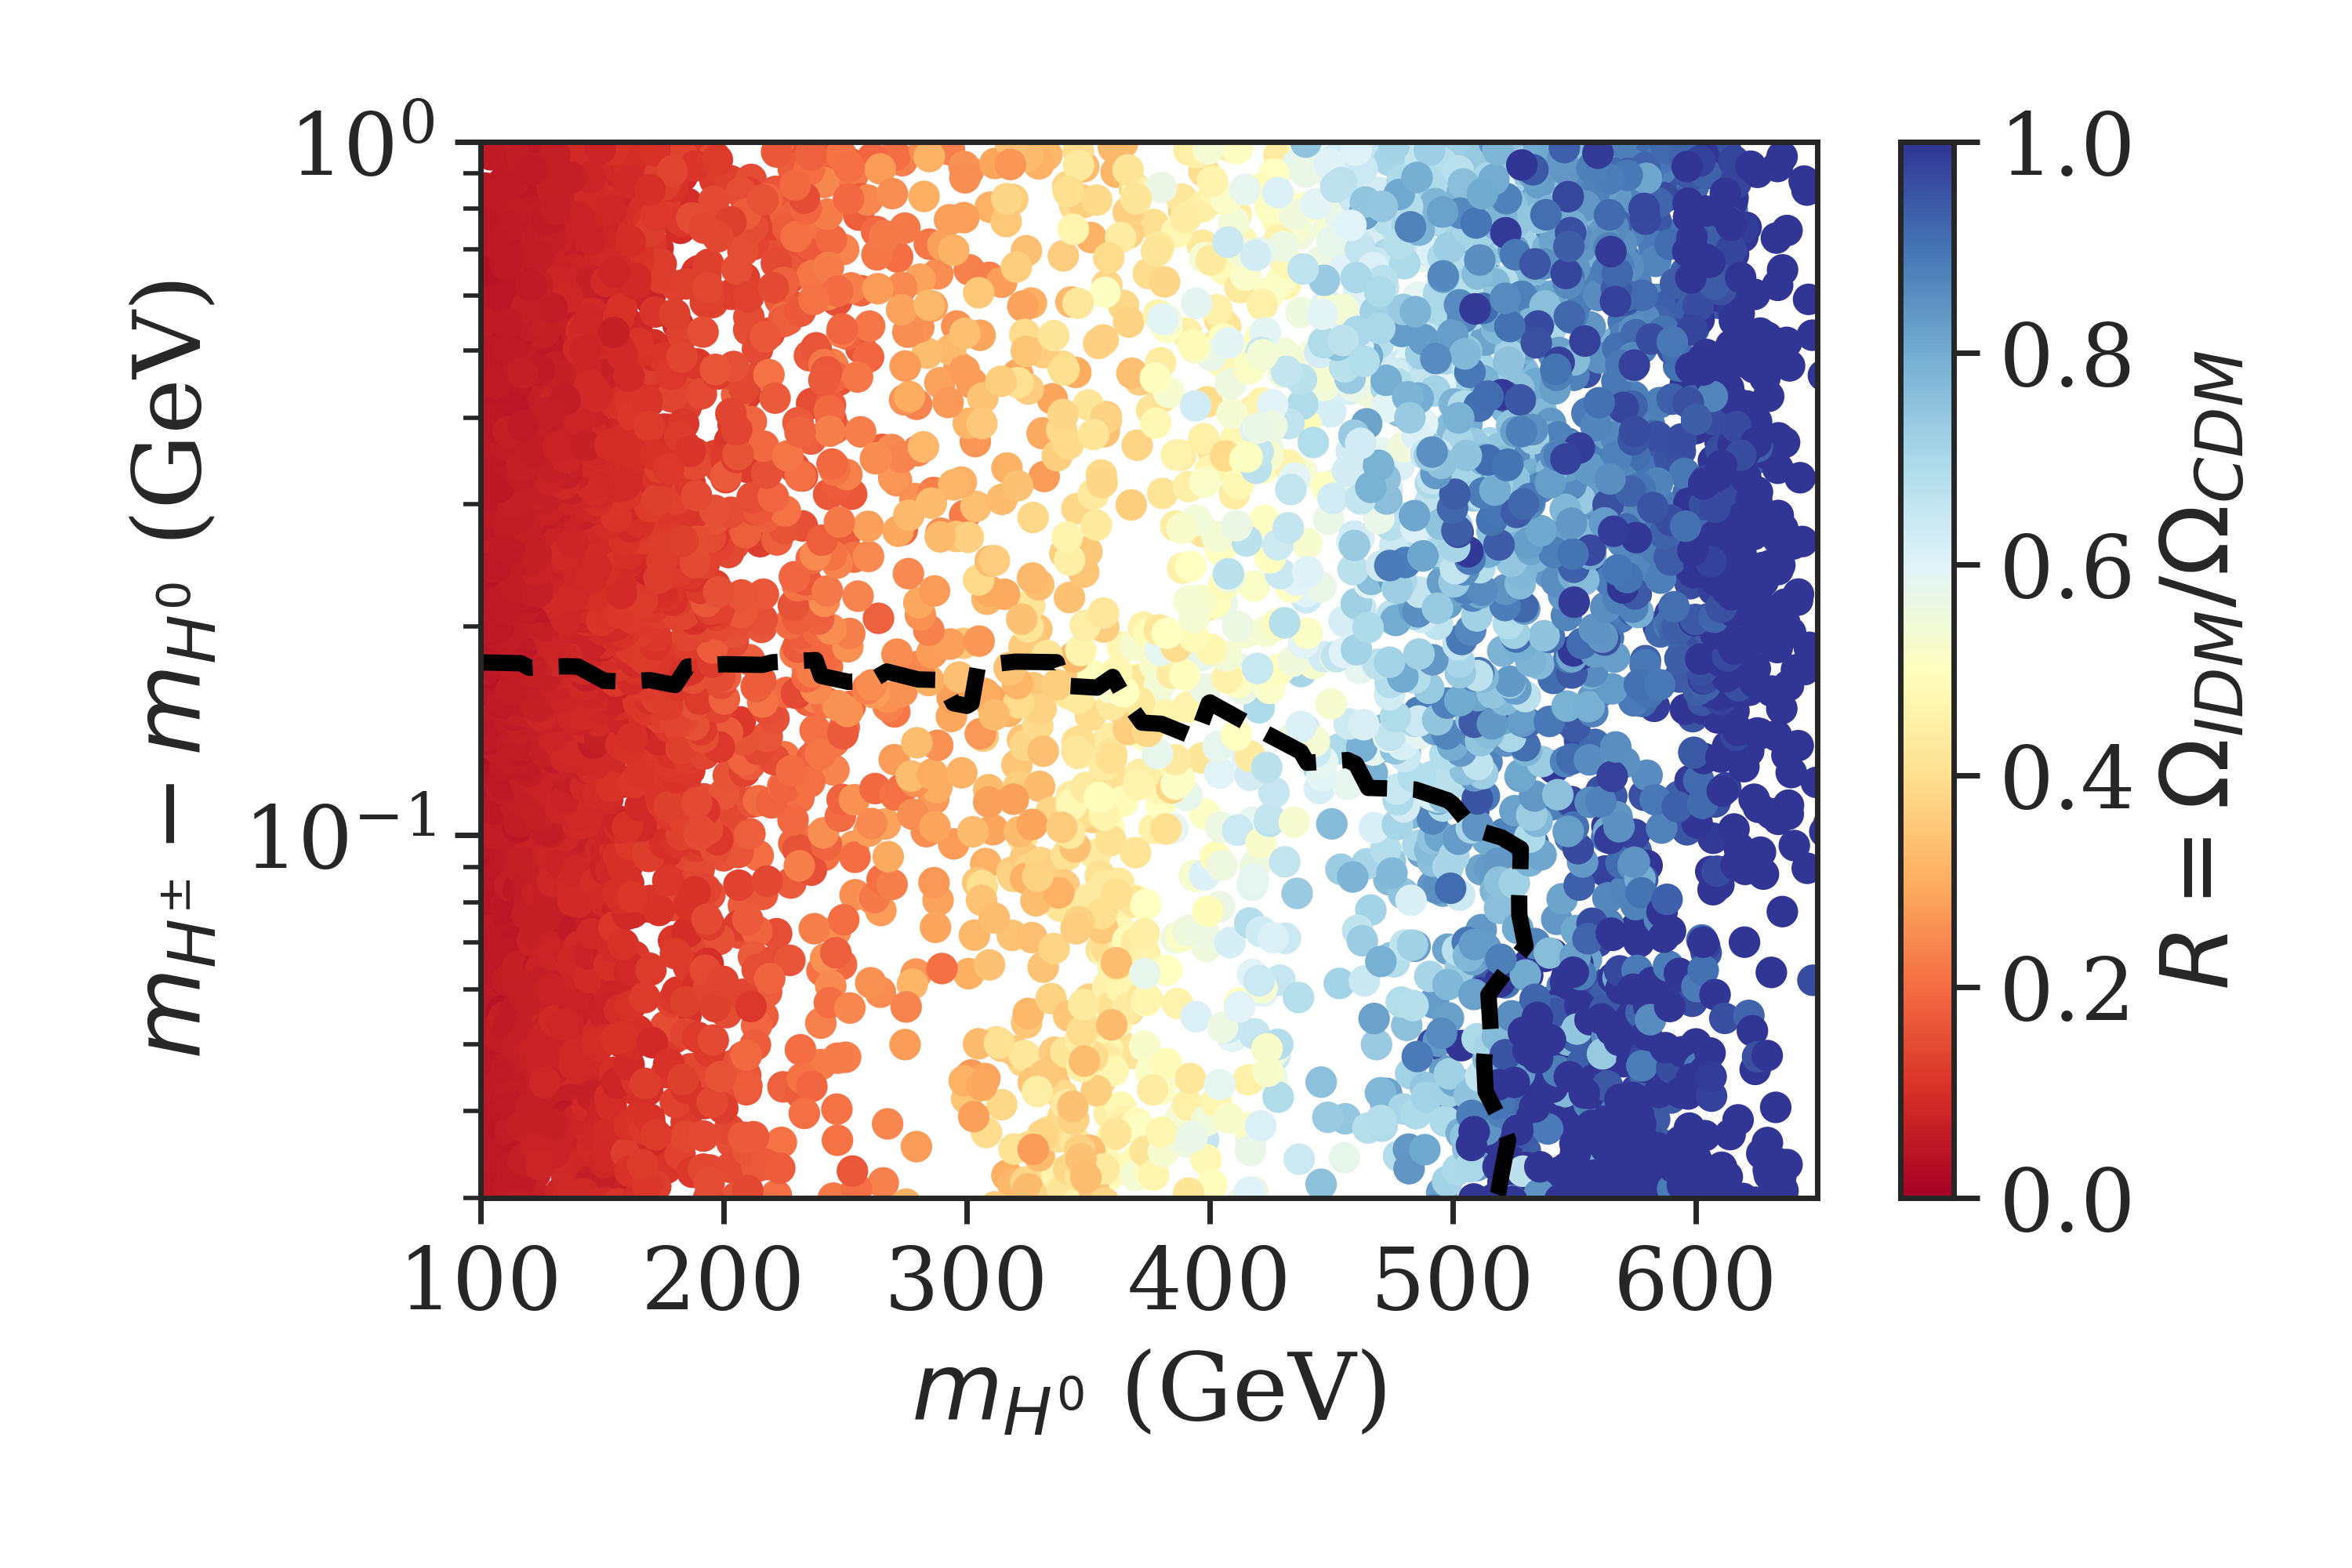
\includegraphics[clip, trim={0cm 0.6cm 0cm 0cm}, width=0.48\textwidth]{figures/IDM_relicRatio_deltaM.png}}
\end{picture}
\caption{Allowed IDM parameter points (imposing all but the LHC constraints) in the $m_{\Hp}$-$c\tau$ plane (left panel) and
$m_{\Hp}$-$\Delta m$ (right panel). The color denotes the
LHC signal strength $r$ and the dark matter fraction $R$, respectively. The black dashed curve shows the
(interpolated) 95\% CL exclusion contour from the LHC ($r=1$).
}
\label{fig:idmres}
\end{figure*}
%                                      \         |
%                                        \       |
%                                          \     |
%=======================


The IDM is a two-Higgs doublet model with an exact ${\cal{Z}}_2$ symmetry, 
under which all standard model fields (including the Higgs doublet $H$) 
are assumed to be even, while the second scalar doublet $\Phi$ is odd. 
It supplements the standard model Lagrangian by the gauge kinetic terms for $\Phi$ as well as
additional terms in the scalar potential, which now reads
\begin{equation}
\begin{split}
	V = &\;\mu_1^2 |H|^2  + \mu_2^2|\Phi|^2 + \lambda_1 |H|^4+ \lambda_2 |\Phi|^4 \\
	&+ \lambda_3 |H|^2| \Phi|^2
		+ \lambda_4 |H^\dagger\Phi|^2 \\
		&+ \lambda_5/2\,\big[ (H^\dagger\Phi)^2 + \mathrm{h.c.} \big].
\label{Eq:TreePotential}
\end{split}
\end{equation}
After electroweak symmetry breaking the model contains five physical scalar states with masses given by
\begin{equation}
\begin{split}
	&m_{\hn}^2 = \mu_1^2 + 3 \lambda_1 v^2\,,\quad
	m_{\Hn}^2= \mu_2^2 + \lambda_L v^2\,, \\ 
	&m_{\An}^2 = \mu_2^2 + \lambda_S v^2\,,\quad
	m_{\Hp}^2 = \mu_2^2 + \frac{1}{2} \lambda_3 v^2\,.
\end{split}
\end{equation}
where
\begin{equation}
	\lambda_{L,S} = \frac{1}{2} \left( \lambda_3 + \lambda_4 \pm \lambda_5 \right)\,,
\end{equation}
After imposing $m_{\hn} \simeq 125.09$\,GeV~\cite{pdg}, we are left with five free physical parameters: $m_{\Hn}$, $m_{\An}$, $m_{\Hp}$, $\lambda_L$ and $\lambda_2$.



Despite its simplicity, the IDM leads to a rich phenomenology and provides a viable dark matter candidate
with observable signatures in direct and indirect detection experiments. For recent accounts 
see \emph{e.g.}~\cite{Ilnicka:2015jba,Belyaev:2016lok,Eiteneuer:2017hoh}. 
At the LHC the IDM is extremely difficult to observe via MET searches~\cite{Pierce:2007ut,Cao:2007rm,Dolle:2009ft,Miao:2010rg,Gustafsson:2012aj,Belanger:2015kga}. For instance, a reinterpretation of dilepton plus MET signatures at the 8\,TeV LHC~\cite{Aad:2014vma}
provides sensitivity up to $m_{\Hn}\simeq 55\,$GeV only~\cite{Belanger:2015kga}. 
However, in this low-mass region, the $\Hn$ thermal relic density ($\Omega_{\text{IDM}}$) is above
the observed dark matter density ($\Omega_{\text{CDM}}$).
There are three regions where the IDM can account for the entire observed relic density ($55\,\text{GeV}\lesssim m_{\Hn} \le m_{h^0}/2$, $m_{\Hn}\simeq72\,\text{GeV}$ and $m_{\Hn}\gtrsim 500\,\text{GeV}$) and a region where it can account only for a fraction of $\Omega_{\text{CDM}}$  ($72 \lesssim m_{\Hn} \lesssim 500\,\text{GeV}$)~\cite{Goudelis:2013uca,Eiteneuer:2017hoh}.

In this work we focus on the region with small mass splittings ($\Delta m = m_{\Hp} - m_{\Hn} \le1\,\text{GeV}$) and use \smo~1.2 to reinterpret the LHC limits from HSCP searches within the IDM model. 
For this purpose we perform a scan over the IDM 5-dimensional parameter space restricted to:
\bea
100 \GEV \le & \!m_{H^0} \!&\le1\TEV \nonumber \\
m_{H^0} < & \!m_{A^0} \!& \le1.1\TEV \nonumber \\
10\MEV \le & \!m_{H^\pm} -m_{H^0}\!& \le1\GEV \nonumber \\
-4\pi \le &  \lambda_L  & \le 4\pi  \\
10^{-6} \le &  \lambda_2  & \le 4\pi \nonumber
\eea
and we impose $10^{-3} \leq R \equiv \Omega_{\text{IDM}}/\Omega_{\text{CDM}} \leq 1$.
In addition we take into account constraints from Higgs invisible decays~\cite{Aad:2015pla}, 
electroweak precision observables~\cite{Baak:2014ora,Eriksson:2009ws}, from searches for charginos and neutralinos at LEP-II~\cite{Pierce:2007ut,Lundstrom:2008ai}.
indirect detection limits from  $\gamma$-ray observations of dwarf spheroidal galaxies~\cite{Fermi-LAT:2016uux}
and theoretical constraints on unitarity, perturbativity and vacuum stability computed with \textsc{2HDMC}~\cite{Eriksson:2009ws} (see Ref.~\cite{Eiteneuer:2017hoh} for further details\footnote{With respect to Ref.~\cite{Eiteneuer:2017hoh}, in this work we update 
    direct detection constraints additionally imposing the 90\% CL upper limits on the spin-independent
    dark matter-nucleon scattering cross-section recently obtained by Xenon1T~\cite{Aprile:2018dbl}.
}).
In the following we only consider points allowed within the $2\sigma$ region of the above constraints.
We use the nested-sampling algorithm \textsc{Multinest}~\cite{Feroz:2008xx,Feroz:2013hea} 
to efficiently explore the parameter space. 

For the allowed parameter space we compute the decay tables and production cross-sections
with \textsc{MadGraph5\_aMC@NLO}~\cite{Alwall:2014hca} and compute the LHC constraints with \smo~1.2. 
For each parameter space point the constraining power of LHC
searches can be conveniently parametrized by the ratio of the relevant signal cross-section ($\sigma_{th}$) to the corresponding analysis upper limit ($\sigma_{UL}$): $r = \sigma_{th}/\sigma_{UL}$ (see Ref.~\cite{Ambrogi:2017neo} for more details).
If $r \geq 1$ for at least one analysis we consider the point as being excluded.



The results are shown in Fig.~\ref{fig:idmres}.
In the left panel we display the signal strength $r$
in the $m_\Hp$-$c\tau_{H^\pm}$ plane, while the right panel shows
the dark matter fraction $R$ in the $m_\Hn$-$\Delta m$ plane.
Although $r$ does in principle depend on all the model parameters,
we can see that it is mostly driven by the charged Higgs mass and its lifetime. We hence show an approximate exclusion curve in
the plot (dark dashed curve). 
In all the parameter space considered we have verified that
the exclusion is completely dominated by the HSCP searches and even though the \smo\ MET constraints were also applied, they could not
exclude any of the points.
As seen in Fig.~\ref{fig:idmres}, in the quasi-stable limit ($c\tau\gtrsim10^3\,$m) HSCP searches exclude $\Hp$ masses up to 580\,GeV.
This limit goes beyond the 13\,TeV LHC limit for direct production of detector-stable staus which reaches 
$m_{\tilde\tau} = 360\,$GeV~\cite{CMS-PAS-EXO-16-036}. The reason for the higher reach is the appearance of 
the additional $W$-mediated production channel $p p \to \Hn\Hp$ as well as (to a lesser extend and depending on $m_{\An}$)
the channels $p p \to \An\Hp, \An \An$ with  $\An\to\Hp$.
As an example, for $m_{\Hn} \simeq m_{\An} \simeq m_{\Hn} \simeq 520$~GeV
we have $\sigma(\Hp \Hp) + \sigma(\Hp \Hn) + \sigma(\Hp \An) \simeq 1.14$~fb against $\sigma(\tilde\tau\tilde\tau) \simeq 0.15$~fb~\cite{CMS-PAS-EXO-16-036} for the same stau mass.

At the lower edge of our scan range, for $m_\Hp\simeq m_\Hn\gtrsim100\,$GeV, HSCP searches are able to constrain
decay lengths down to around $c \tau \simeq 2\,m$.
Here the significant exponential suppression of ${\cal F}_\text{long}$ is
compensated by the large cross-section. Note that our choice for $\langle\ell_\text{outer}/\gamma\beta\rangle_\text{eff}$
leads to a somewhat conservative exclusion limit in this part of the parameter space (see left panel of Fig.~\ref{fig:leff}
as well as the corresponding discussion in \ref{app:lifetime}). 
We point out that the calculation of $ c\tau$ involves a certain degree of approximation. First, the decays are computed at leading order with \textsc{MadGraph5\_aMC@NLO} and the decay channels with first generation quarks in the final state are turned off once $\Delta m$ is smaller
than the pion mass.
This introduces the (artificial) gap seen at $c \tau \sim 100$~m, which would not appear if the proper phase-space including the pion mass were included.



In the right panel of Fig.~\ref{fig:idmres} we show the HSCP exclusion curve in the $\Delta m$-$m_{\Hn}$ plane.
As seen, the limits exclude a significant part of the parameter space with $\Delta m \lesssim 0.2\,$ GeV. Interestingly, the HSCP searches are starting to exclude part of the region with $R=1$, where the IDM can account for the entire observed relic density ($m_{\Hn} \gtrsim 500$~GeV). 
Note that disappearing track searches have the potential to further extend the reach towards larger $\Delta m$~\cite{Belyaev:2016lok}.  

%----------------------------------------------------------------------------------------------------------------
\subsection{Gravitino dark matter scenario}\label{sec:grav}
%----------------------------------------------------------------------------------------------------------------

The gravitino -- the superpartner of the graviton -- is an attractive dark matter candidate in supersymmetric theories~\cite{Fayet:1981sq,Pagels:1981ke}. Models where the gravitino ($\tilde G$) is the LSP can alleviate the gravitino problem
%\cite{Weinberg:1982zq,Ellis:1984eq,Falomkin:1984eu,Ellis:1984er}
which appears in neutralino LSP scenarios~\cite{Weinberg:1982zq,Ellis:1984eq,Falomkin:1984eu,Ellis:1984er}
unless the gravitino is much heavier than the rest of the supersymmetric spectrum which in turn severely limits the viable options for supersymmetry breaking.
Once the gravitino is the LSP, the lightest sparticle of the MSSM (\emph{i.e.}~the NLSP) can be any sparticle. However, in order to not reintroduce a severe problem through
late decays of the NLSP -- spoiling successful BBN predictions~\cite{Moroi:1993mb} -- certain choices
appear more promising. For instance, the stau is an attractive NLSP candidate  providing a large annihilation cross-section, thus resulting in smaller freeze-out abundances. As a consequence, the impact of the late time decay $\tilde{\tau} \to \tau \tilde G$ on BBN is reduced.
On the other hand it also reduces the contribution to the gravitino abundance through NLSP decays. This allows for a larger thermal contribution of gravitino production while not over-closing the Universe. Since the thermal contribution is (approximately) proportional
to the reheating temperature, $\Omega^{\text{th}}_{\s G}\propto T_\text{R}$~\cite{Bolz:1998ek,Bolz:2000fu,Pradler:2006hh},
it allows for higher values of $T_\text{R}$, as preferred by classes of models for leptogenesis and
inflation\com{REFS?}.


Here we revisit the parameter scan performed in~\cite{Heisig:2013rya,Heisig:2013sva} refining and updating the 
constraints from long-lived particle searches at the LHC\@. 
%In~\cite{Heisig:2013rya} searches for HSCPs and 
%$R$-hadrons at the the 8\,TeV LHC have been taken into account. The %respective constraints from HSCP
%have been computed in an approximate way using the efficiencies from the %direct production channel and
%the gaugino mediated supersymmetry breaking model as representative benchmarks. 
%        \                                       |
%We consider the pMSSM\@. 
The scan is performed within the framework of the pMSSM, where
the additional assumption $ m_{\s q_{1,2}}\equiv m_{\s Q_{1,2}}=  m_{\s u_{1,2}}\!= m_{\s d_{1,2}}$ has been imposed. In this way we
achieve a 17-dimensional parameter space with input parameters and scan ranges given by:\footnote{In this phenomenologically driven parameter scan the spectrum parameters of the third generation sfermions, 
$\mstau, \,m_{\tilde{t}_1}, \,m_{\tilde{b}_1}, \,\thest$ and $ \theta_{\tilde{t}}$, were 
chosen as input parameters in order to obtain an equally good
coverage of small and large mixing scenarios. Tree-level relations were used to translate these 
parameters into soft parameters. In the further analysis only the values recalculated by the spectrum 
generator are used consistently.}
\bea
-10\TEV \le &A_t &\le10\TEV \nonumber \\
-8\TEV \le &A_b,\,A_\tau, \mu& \le8\TEV \nonumber \\
1 \le & \tan\beta & \le 60 \nonumber \\
100\GEV \le &  m_A  & \le 4\TEV \nonumber \\
200\GEV \le & \mstau & \le 2\TEV \nonumber \\
700\GEV \le & m_{\tilde{t}_1}, m_{\tilde{b}_1} & \le 5\TEV \label{eq:scanranges}\\
0 < &  \thest, \theta_{\tilde{t}} & < \pi \nonumber \\
\mstau  \le & \!\!m_{\s L_{1,2}}, m_{\s e_{1,2}} \!\!& \le  4\TEV \nonumber \\
1.2\TEV\le & \!\!m_{\s q_{1,2}}\!\!
%=  m_{\s u_{1,2}}\!= m_{\s d_{1,2}}\!\! 
& \le  8\TEV \nonumber \\
\mstau  \le &  M_1, M_2 & \le  4\TEV \nonumber \\
1\TEV \le & M_3 & \le  5\TEV \nonumber 
\eea
The particle spectrum has been computed with \textsc{SuSpect}~2.41 \cite{Djouadi:2002ze}
and \textsc{FeynHiggs}~2.9.2~\cite{Heinemeyer:1998yj}. 
Since we are interested in the gravitino LSP scenario with a stau NLSP, we have required all the points to have the lighter stau $\stau_1$ as the NLSP. In addition we have also imposed $m_h  \in [123;128]\GEV$~\cite{pdg,Degrassi:2002fi}.

The decay widths and branching ratios have been computed with 
\textsc{SDecay}~\cite{Djouadi:2006bz,Kraml:2007sx} and (in the case of missing dominant decay channels) \textsc{MadGraph5\_aMC@NLO}~\cite{Alwall:2014hca}, while
the freeze-out abundance of staus have been computed with \textsc{micrOMEGAs}~2.4.5~\cite{Belanger:2008sj}.
We considered constraints on the MSSM Higgs sector\com{The end of the paragraph also mentions MSSM Higgs sector constraints. Clarify?}, performed at LEP, the Tevatron and the LHC~\cite{Bechtle:2011sb}
and EW precision bounds~\cite{Group:2012gb,Bechtle:2012jw,Heinemeyer:2006px} as well as
theoretical constrains arising from charge or color breaking vacua~\cite{Kitahara:2013lfa,Frere:1983ag,AlvarezGaume:1983gj,Claudson:1983et,Kounnas:1983td,Derendinger:1983bz}. With respect to~\cite{Heisig:2013rya} we imposed updated flavor constraints: $\text{BR}(B\to X_s\gamma) \in [3.0;3.64]\times 10^{-4}$ 
\cite{Amhis:2016xyh} and 
$\text{BR}(B_s^0\to\mu^+\mu^-) \in [1.74;4.34] \times 10^{-9}$~\cite{Aaij:2017vad}.
Finally, limits on the MSSM Higgs sector were included by applying the conservative constraints on $m_A$ and $\tan\beta$
derived in the $m_h^{\text{mod}+}$-scenario~\cite{Sirunyan:2018zut}. 

Since the gravitino mass can be taken as an additional free parameter, for each point in the pMSSM parameter space satisfying the above requirements, 10 gravitino masses have been generated. The randomly selected values were required to lie within an interval where the total $\tilde G$ abundance can match the measured dark matter abundance: 
\begin{equation}
\label{eq:Omcont}
\Omega_{\s G}^{\text{non-th}} h^2+\Omega^{\text{th}}_{\s G}h^2  = \Omega_\text{CDM}h^2\,,
\end{equation}
where $\Omega^{\text{th}}_{\s G}h^2$ and $\Omega_{\s G}^{\text{non-th}} h^2$ are the thermal and non-thermal gravitino relic abundances, respectively.
The latter is generated once the frozen-out $\tilde{\tau}$s decay to $\tilde G$s,
thus enhancing the total gravitino abundance.
On the other hand the thermal gravitino relic abundance is mostly determined by the reheat temperature, $T_\text{R}$~\cite{Bolz:1998ek,Bolz:2000fu,Pradler:2006hh}.
Therefore, given a pMSSM point (and hence $\Omega_{\s G}^{\text{non-th}} h^2$), the reheating temperature is computed imposing \eqref{eq:Omcont} with $\Omega_\text{CDM}h^2=0.1189$. %~\cite{Ade:2013zuv}.
For each of the resulting points in the (17+1)-dimensional parameter space (that by construction fulfills the
relic density constraint) constraints from BBN~\cite{Jedamzik:2007qk,Jedamzik:2006xz}\footnote{Furthermore, constraints from diffuse gamma ray
observations~\cite{Sreekumar:1997yg,Kribs:1996ac} have been considered, which, however, have found to be much less relevant~\cite{Heisig:2013sva}.}
have been imposed (see Refs.~\cite{Heisig:2013rya,Heisig:2013sva} for further details).
% which depend on the freeze-out abundance, the lifetime and the hadronic branching ratios
%of the stau decaying into the gravitino.
%The latter have been computed with the spin-$3/2$ extension of \textsc{MadGraph}~\cite{Hagiwara:2010pi,Alwall:2007st}. For further details we refer to~\cite{Heisig:2013rya,Heisig:2013sva}.


\begin{figure}[t]
    \centering
    \setlength{\unitlength}{1\textwidth}
    \begin{picture}(1,0.29)
    \put(0.0,-0.003){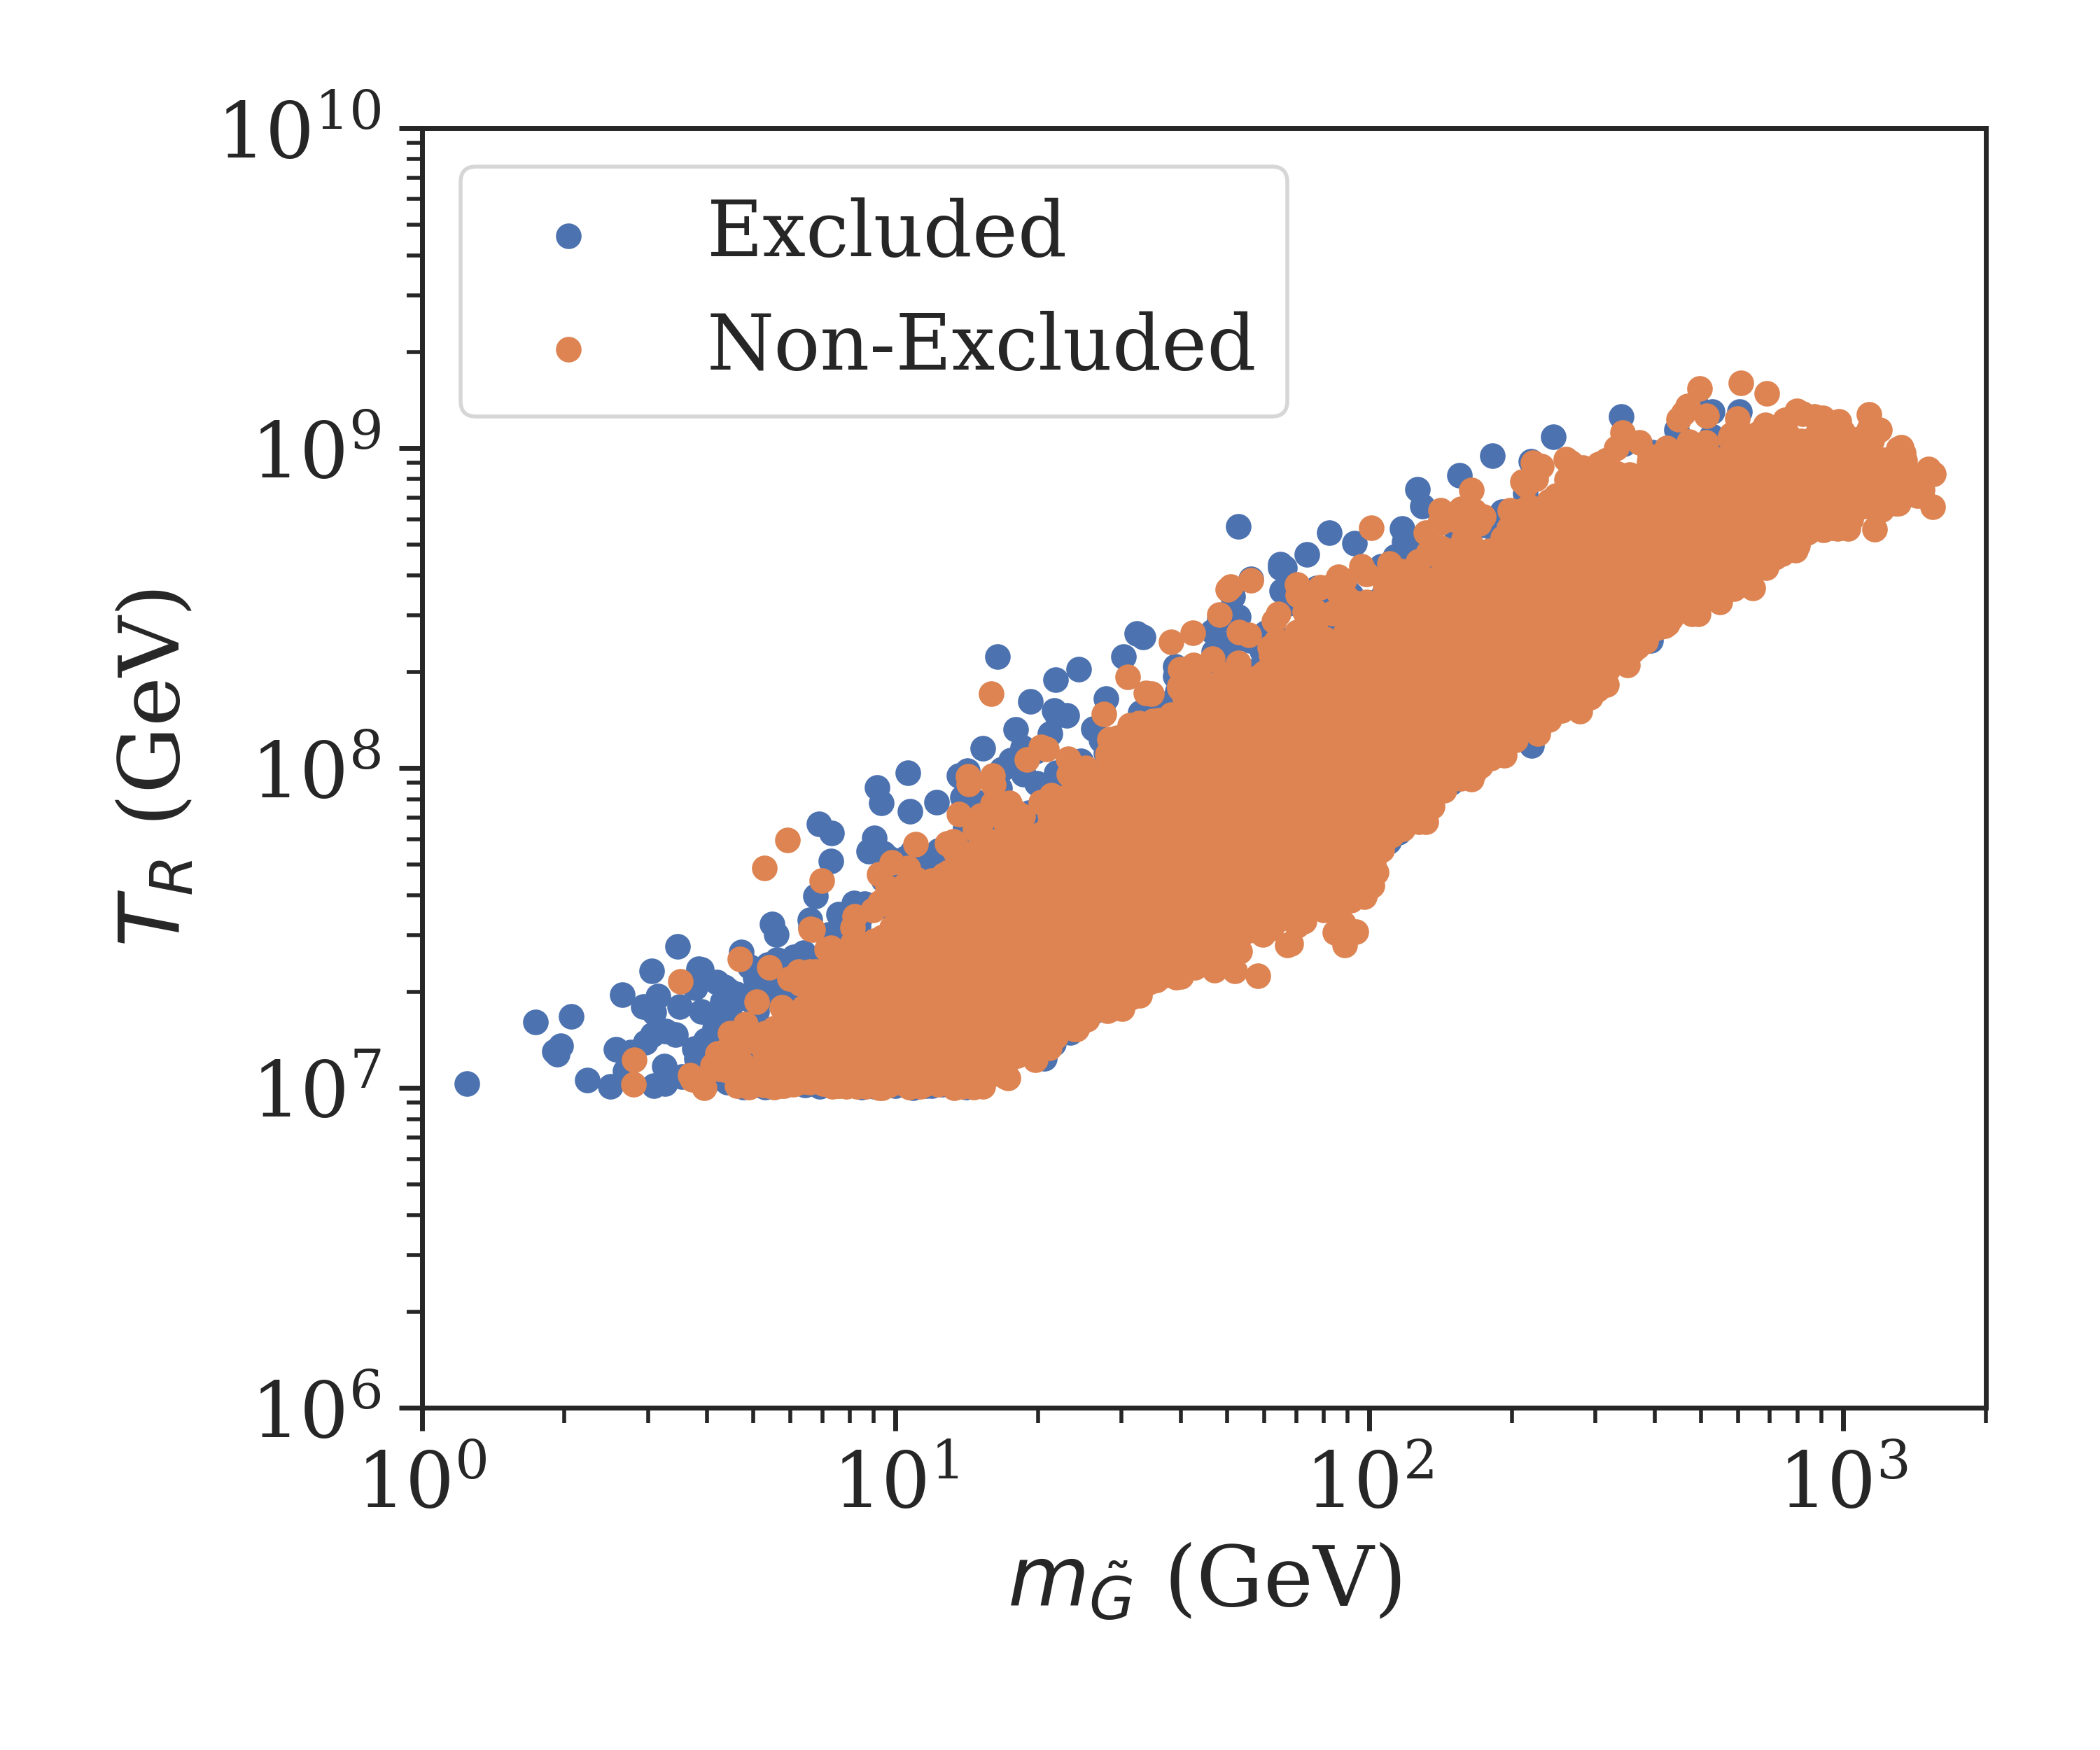
\includegraphics[clip, trim={0cm 0.6cm 0cm 0cm}, width=0.47\textwidth]{figures/Gravitino_all.png}}
    \end{picture}
    \caption{Effect of the LHC exclusion bounds on the otherwise allowed points in the plane spanned by the gravitino mass and reheating temperature.}
    \label{fig:gavitinores1}
\end{figure}
%                                      \         |
%                                        \       |
%                                          \     |
%=======================

After selecting $\sim$26k points satisfying the above constraints,
%(we have 28k points minus ~2k points which fail BBN)
 we have used \smo~1.2 to decompose each point signal into all occurring simplified model topologies, which includes production and cascade
decays of all MSSM supersymmetric particles.
The LO production cross-sections have been computed using \textsc{Pythia}~8~\cite{Sjostrand:2006za,Sjostrand:2014zea}, while
NLL cross-sections for $\tilde g \tilde g$, $\tilde g \tilde q$ and $\tilde q \tilde q$  have been obtained using \textsc{NLLFast}~\cite{Beenakker:1996ch,Beenakker:1997ut,Kulesza:2008jb,Kulesza:2009kq,Beenakker:2009ha,Beenakker:2010nq,Beenakker:2011fu}.
The results from the 8~TeV and 13~TeV HSCP and $R$-hadron searches were then applied in order to constrain the points. Since all the cascade decays terminate at the stau NLSP (at collider scales), MET constraints do not apply. 
From all the tested points, $\sim 5$k are excluded and $\sim 21$k are allowed, as shown in Fig.~\ref{fig:gavitinores1}.
For a fixed gravitino mass (below $\sim 200$~GeV), the largest values of $T_{\text{R}}$ are excluded by the LHC constraints. This is due to the fact that the largest reheat temperatures are typically achieved for points with small gluino masses\com{Explain more?}, which in turn contain large production cross-sections at the LHC. As a result these points can be probed by the HSCP and $R$-hadron searches. We see, however, that the largest values of $T_{\text{R}}$ ($\simeq 10^9$~GeV) obtained in the scan
are still allowed by the LHC constraints obtained with \smo.


In order to discuss which searches and topologies are relevant for testing the gravitino scenario, we show in Fig.~\ref{fig:gavitinores2} a histogram for the number of excluded points as a function of the gluino mass. 
In the left panel the number of excluded points is grouped according to which is the most constraining type of signature. The stacked histogram shows that the bulk of the points are excluded by topologies containing HSCP signatures, as expected.
Nonetheless a significant fraction of points at low $m_{\tilde g}$ are excluded by $R$-hadron constrains for long-lived gluinos. These points typically have heavy squarks, resulting in suppressed 3-body or 4-body gluino decays. In a similar way, points with light squarks and heavy gauginos and higgsinos lead to long-lived squarks which can also be constrained by the $R$-hadron searches, as shown by the orange histogram.
In order to illustrate the constraining power of combining results for multiple simplified model topologies, we also display (dark blue histogram) the distribution of excluded points obtained using only the CMS limits for pair production of long-lived staus, gluinos and squarks.
As it can be seen, the number of excluded points in this case ($\sim200$) is drastically reduced when compared to the one obtained with all the topologies included in \smo.


We point out, however, that the constraining power of \smo\ is still limited by the number of simplified model results contained in its database. The points from the pMSSM scan performed here
display a large variety of topologies and many of them do not fall within the 8 HSCP or the 2 $R$-hadron topologies included in the database.
However \smo\ can also be used to identify the most relevant missing topologies~\cite{Kraml:2013mwa,Ambrogi:2017lov,Ambrogi:2017neo}.
In the right panel of Fig.~\ref{fig:gavitinores2}
we show the non-excluded points with a total SUSY production cross-section (at 13~TeV) larger than 5~fb. Due to their sizeable cross-section, such points have a potential for being excluded by the HSCP or $R$-hadron searches. The stacked histogram shows the distribution of non-excluded points as a function of the gluino mass grouped according to the missing topology with largest weight (cross-section times branching ratio). 
Most of the points have  $m_{\tilde g} < 1.7$~TeV, since this ensures $\sigma(\tilde g \tilde g) \gtrsim 5$~fb.
The almost flat distribution at large $m_{\tilde g}$ corresponds to points with light squarks in the spectrum, thus also resulting in large total cross-sections.
We see that the missing topology which occurs more often in Fig.~\ref{fig:gavitinores2} (light blue histogram) corresponds to pair production of BSM particles, which then go through 4-body decays to the HSCP. This topology is mostly generated by points with very light gluinos, which then decay directly to the $\tilde{\tau}$ through 4-body decays.
Furthermore, we see that topologies with 1-step decays to $R$-hadrons (green and dark red histograms) can also be potentially powerful when constraining this scenario. These topologies often appear in points with light quarks (gluinos) which decay to long-lived gluinos (quarks).



%=======================
%    \                                           |
%      \                                         |
%        \                                       |
\begin{figure*}[h]
    \centering
    \setlength{\unitlength}{1\textwidth}
    \begin{picture}(0.96,0.37)
    \put(0.0,-0.00){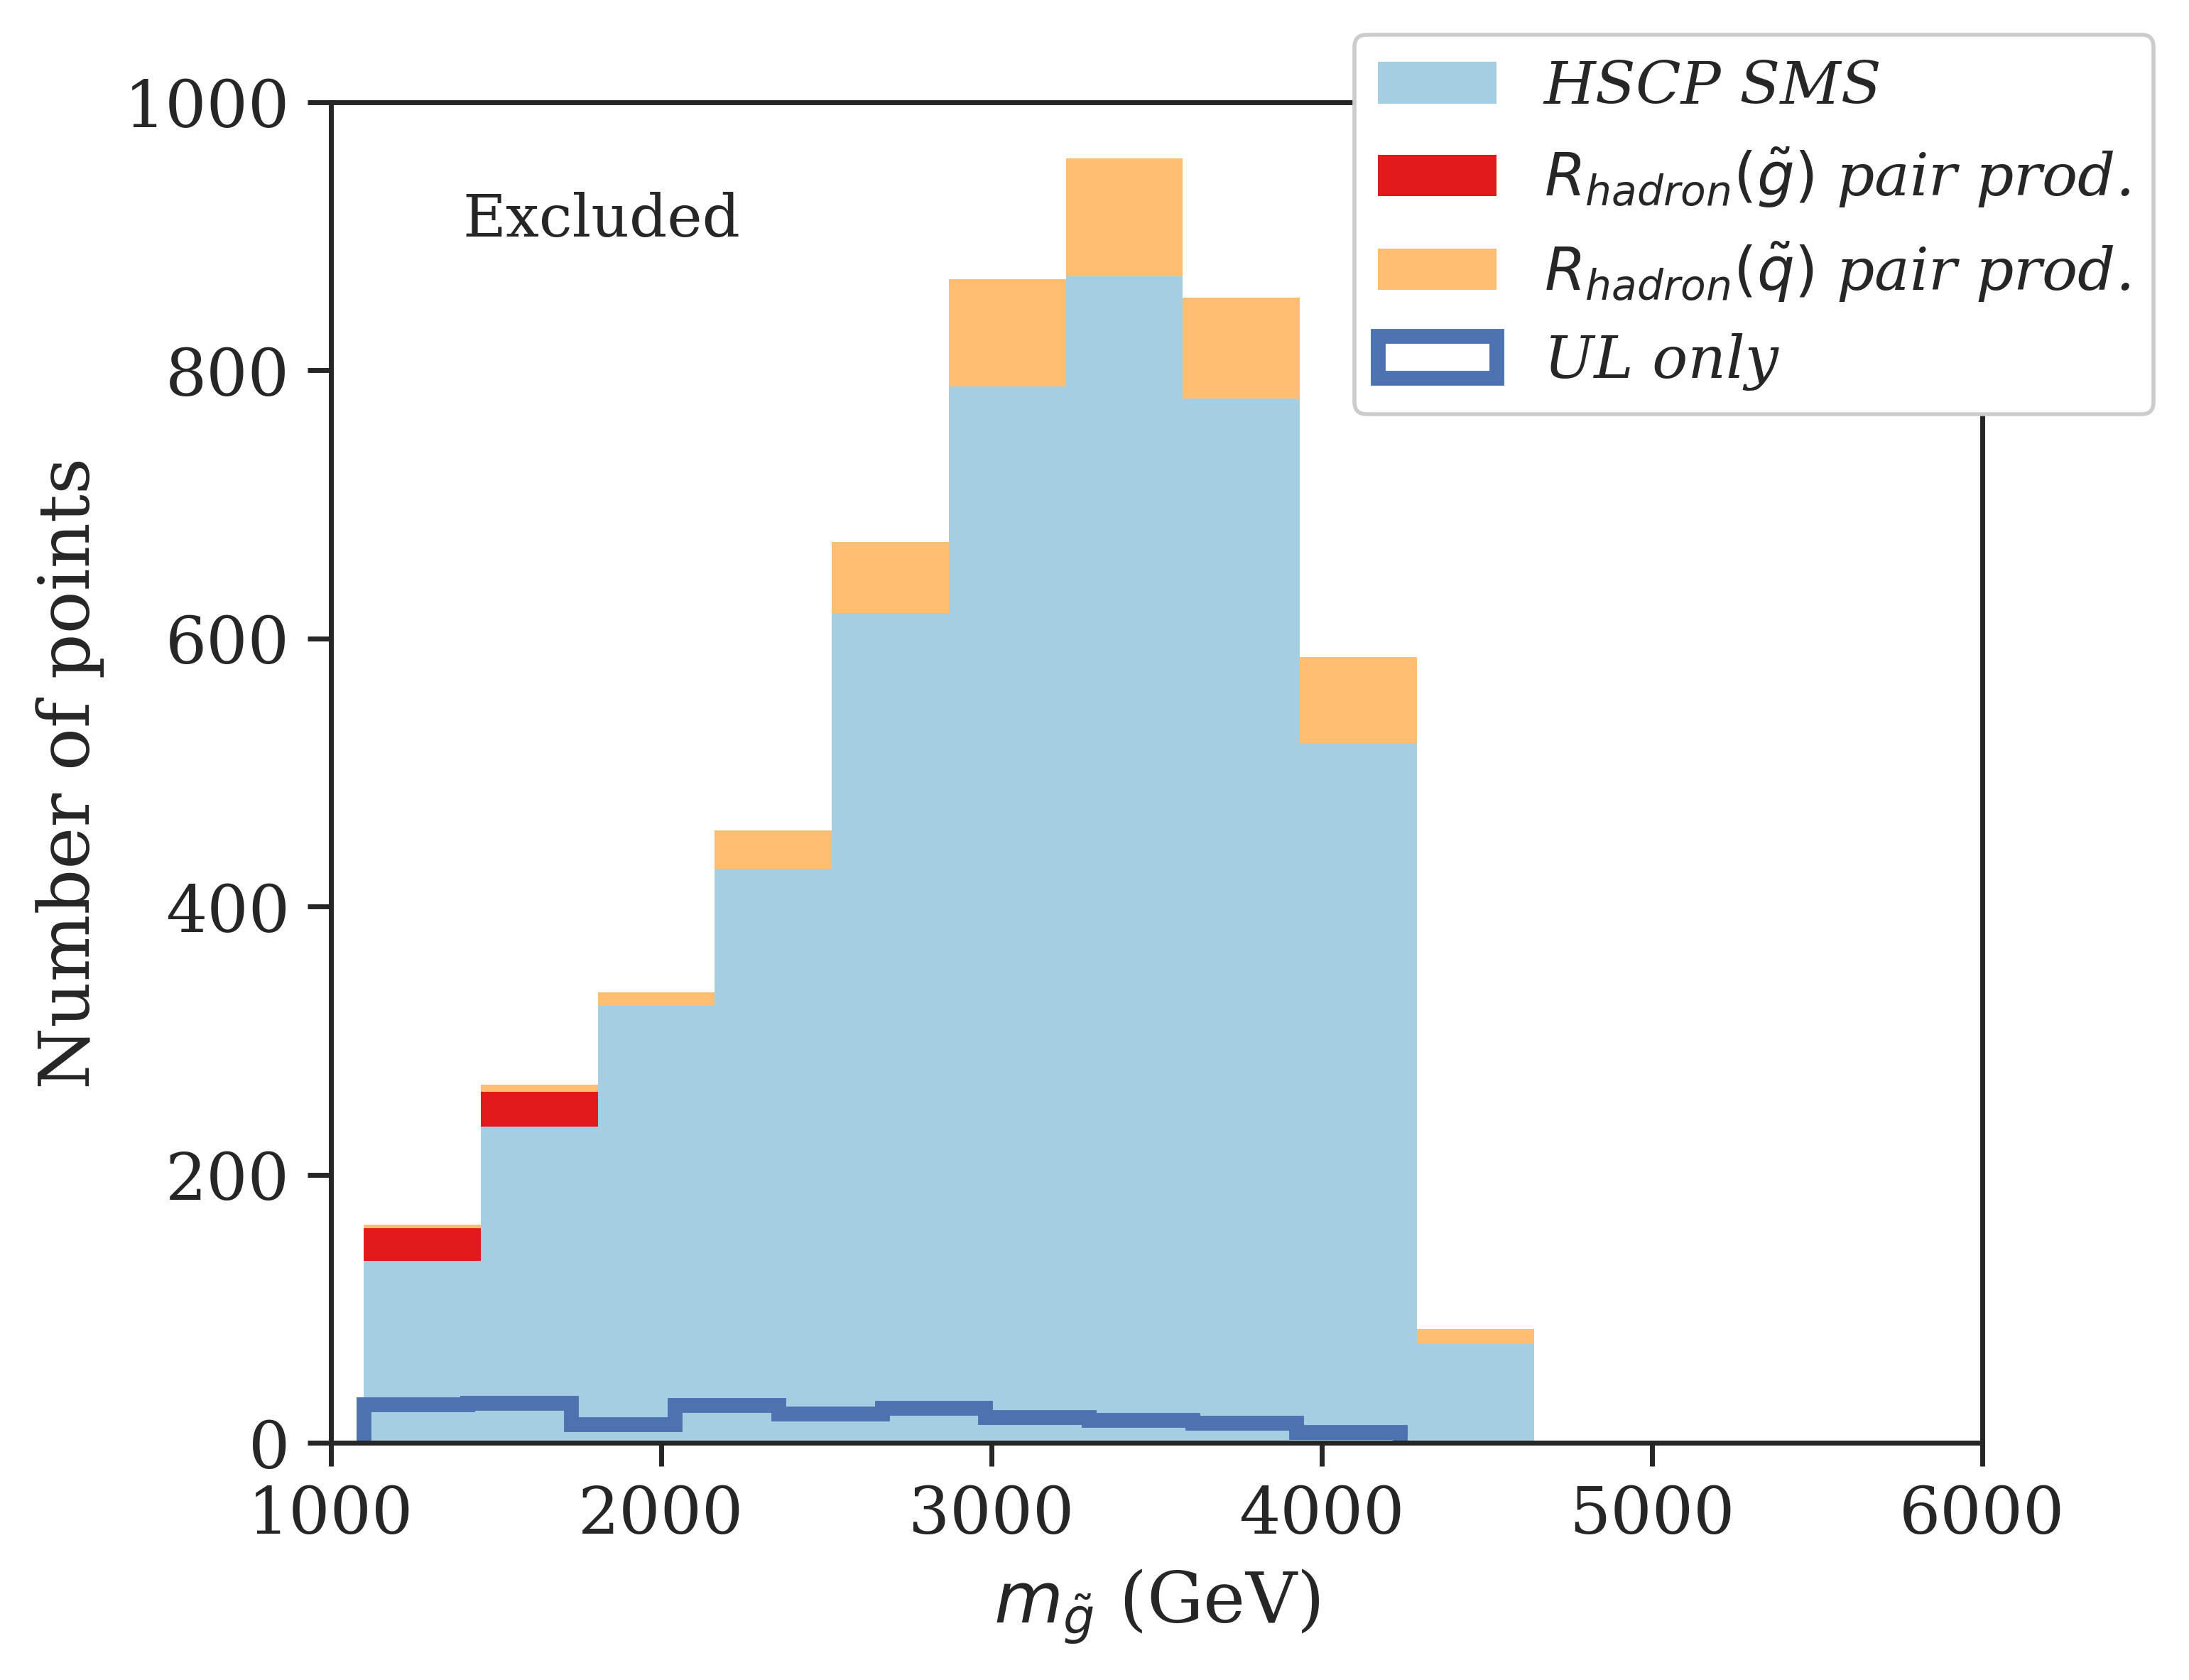
\includegraphics[clip, trim={0cm 0.1cm 0cm 0cm}, scale=0.5]{figures/Gravitino_txnames.png}}
    \put(0.5,0.0){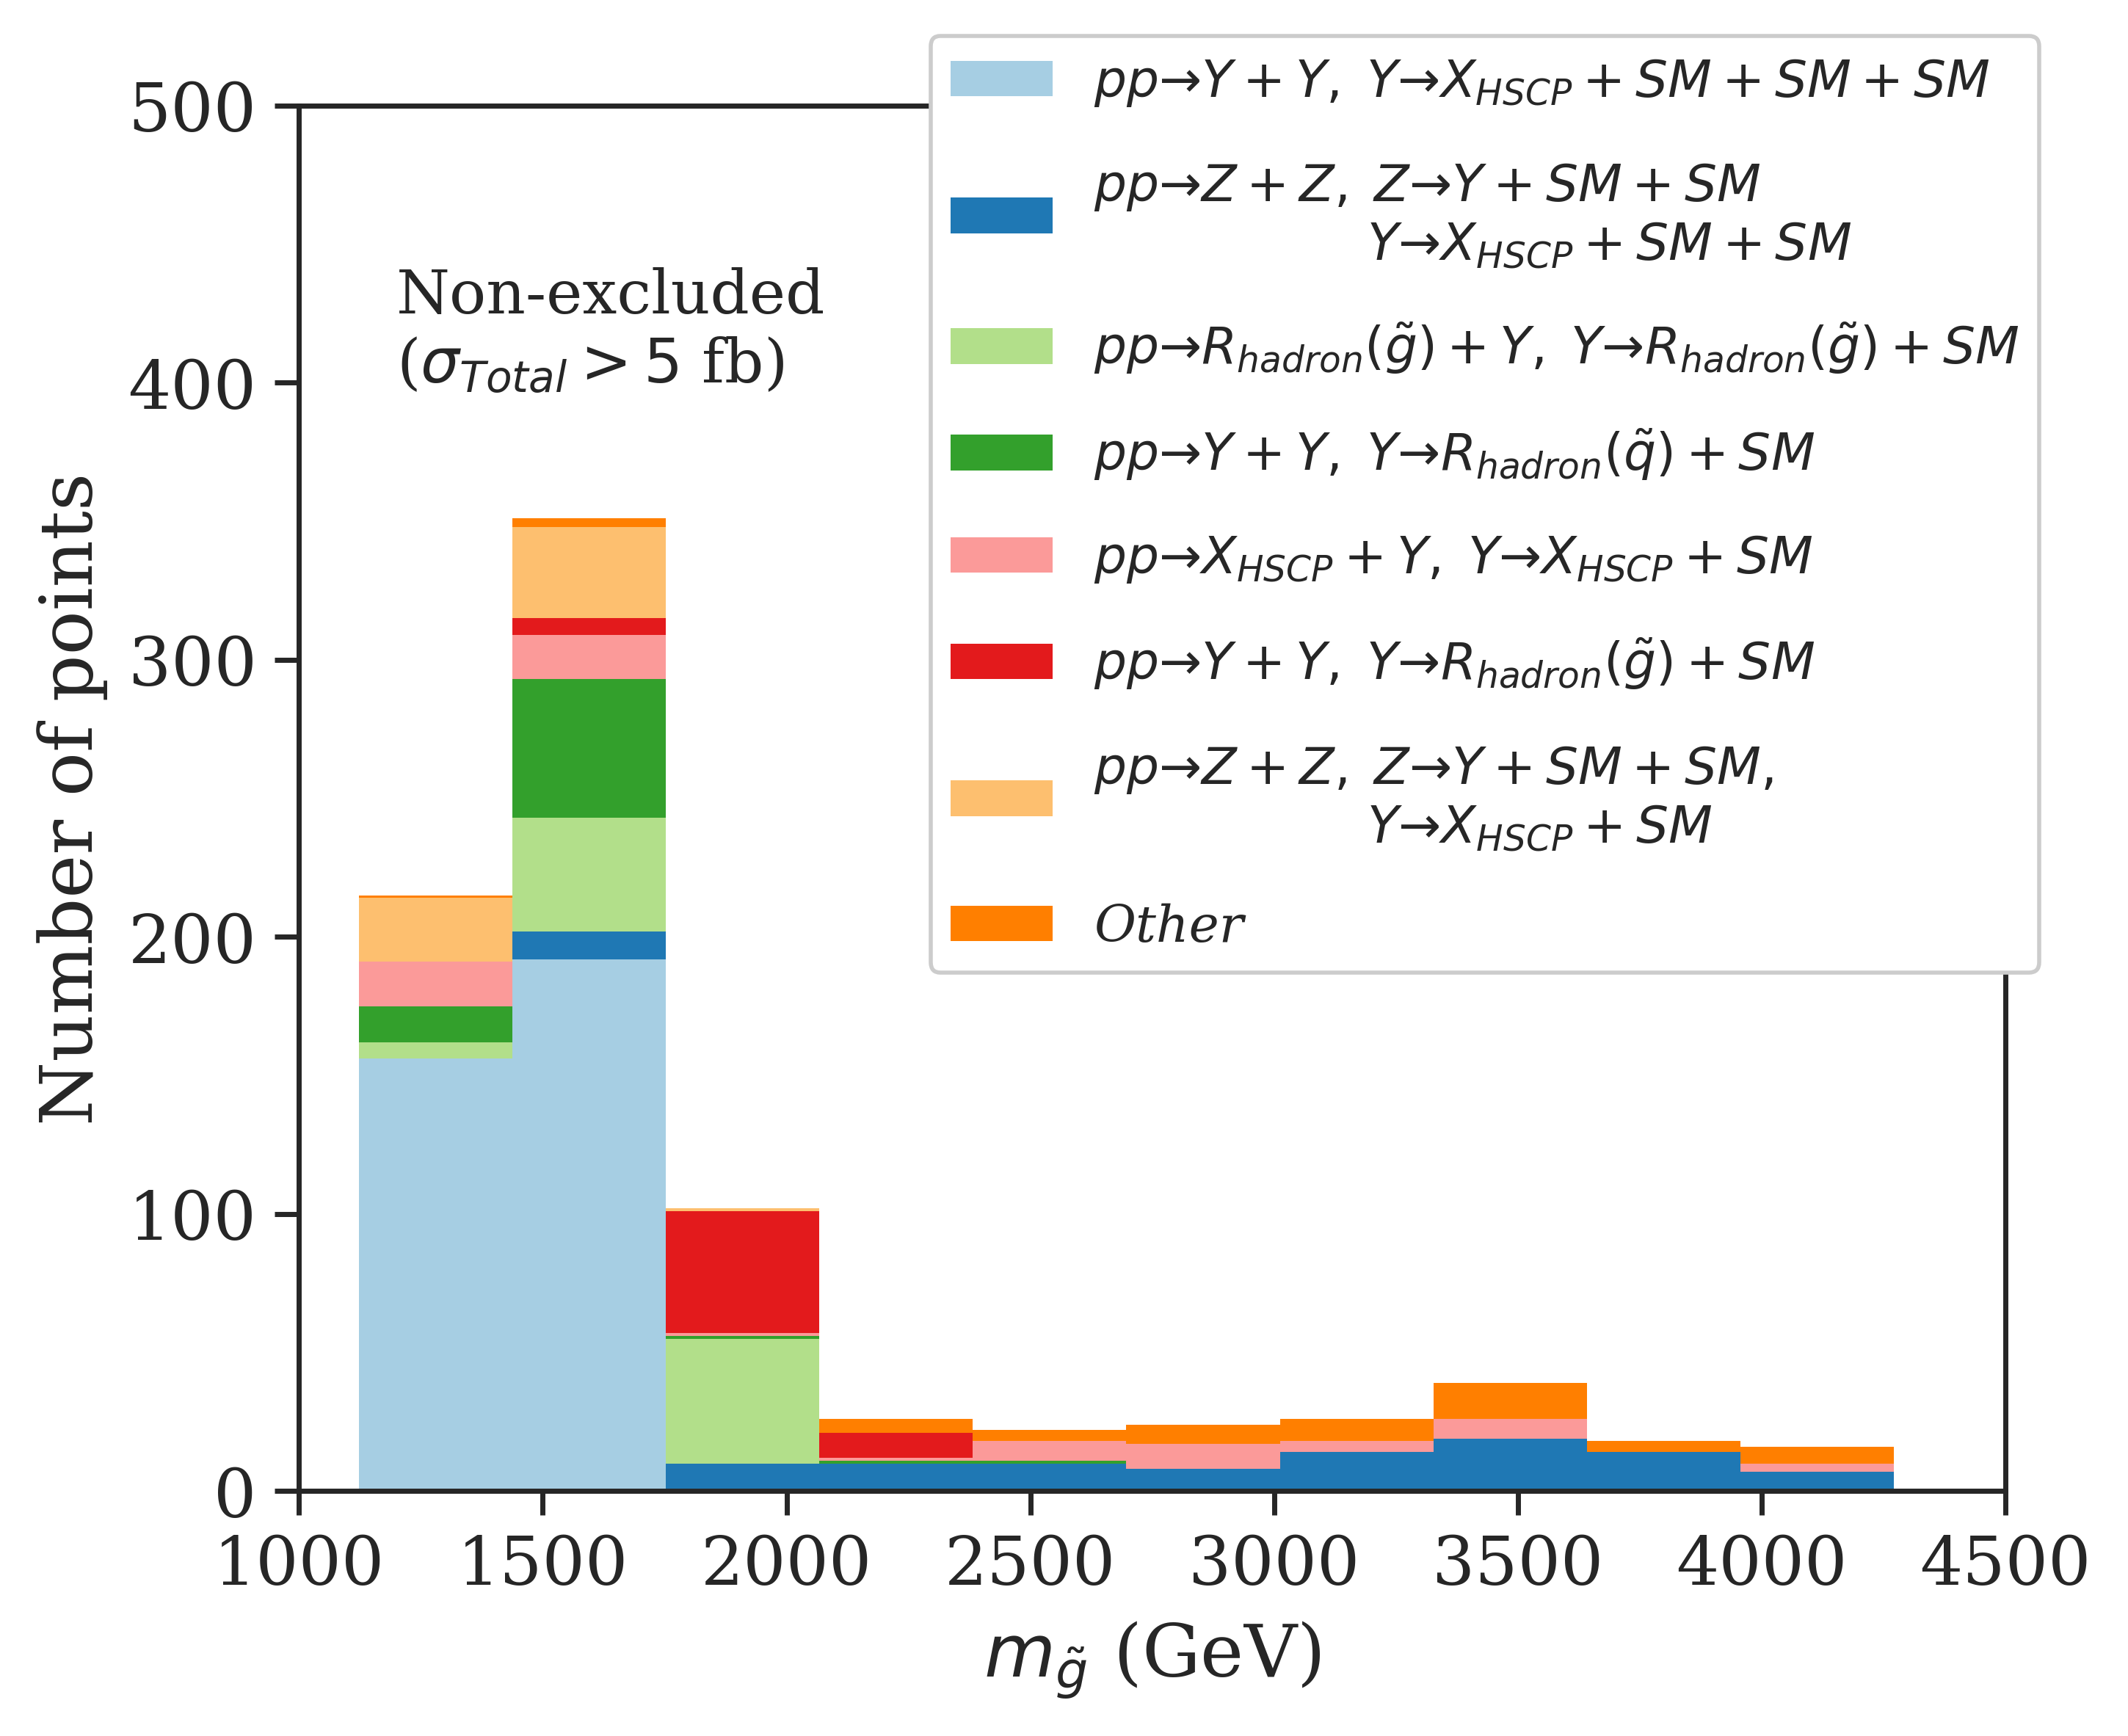
\includegraphics[clip, trim={0cm 0.1cm 0cm 0cm}, scale=0.5]{figures/Gravitino_missedTopos_nonexcluded.png}}
    \end{picture}
    \caption{Left panel: Number of excluded points as a function of the gluino mass. The color indicates the most constraining type of signature. The solid blue histogram displays the number of points excluded when imposing only the CMS limits on the direct pair production of HSCPs and $R$-hadrons.
        Right panel: Number of non-excluded points with a total SUSY production cross-section of more than 5\,fb at 13~TeV. The color indicates the simplified model topology with largest weight (cross-section times branching ratio).}
    \label{fig:gavitinores2}
\end{figure*}
%                                      \         |
%                                        \       |
%                                          \     |
%=======================



% $m_A$
%
%We considered bounds from flavor and precision observables. We applied the constraints 
%$\text{BR}(B\to X_s\gamma) \in [2.87 ; 3.99] \times 10^{-4}$ \cite{HFAGbsgAug12} and 
%$\text{BR}(B_s^0\to\mu^+\mu^-) \in [1.1 ; 6.4] \times 10^{-9}$  \cite{:2012ct} on the respective 
%observables computed by \textsc{micrOMEGAs}~2.4.5~\cite{Belanger:2008sj}. Constraints 
%on the corrections to the mass of the $W$ boson were taken into account by applying the limit 
%$M_W \in [80.325 ; 80.445] \GEV$ \cite{Group:2012gb,Bechtle:2012jw,Heinemeyer:2006px} 
%to the value calculated by \textsc{FeynHiggs}~2.9.2. For the computation of exclusion bounds from collider 
%searches for the MSSM Higgs sector, performed at LEP, the Tevatron and the LHC, we utilized 
%\textsc{HiggsBounds 4.0.0}~\cite{Bechtle:2011sb}.









%===================================================================
\section{Conclusion}\label{sec:summary} 
%===================================================================

In this work we have applied \smo~1.2 to constrain two new physics scenarios containing long-lived particles. This latest \smo version is capable to test BSM models that contain non-neutral long-lived BSM particles. We have implemented HSCP and $R$-hadron
searches at the 8 and 13\,TeV LHC\@. We discuss to benchmark scenarios in order to
illustrate its capabilities, the IDM and a gravitino dark matter scenario.

\com{...}

%----------------------------------------------------------------------------------------------------------------
\section*{Acknowledgements}
%----------------------------------------------------------------------------------------------------------------

We would like to thank Nishita Desai, Suchita Kulkarni and Wolfgang Waltenberger for very helpful discussions.

This work is supported by the German Research Foundation DFG through the 
research unit ``New physics at the LHC''. A.L. is supported by the Sao Paulo Research Foundation (FAPESP), projects 2015/20570-1
and 2016/50338-6. \com{S. Kraml is...}




%%%%%%%%%%%
\begin{appendix}

%===================================================================
\section{Recasting and validation}\label{app:rec13} 
%===================================================================


%=======================
%    \                                           |
%      \                                         |
%        \                                       |
\begin{figure*}[h]
\centering
\setlength{\unitlength}{1\textwidth}
\begin{picture}(0.96,0.3)
\put(0.0,0.0){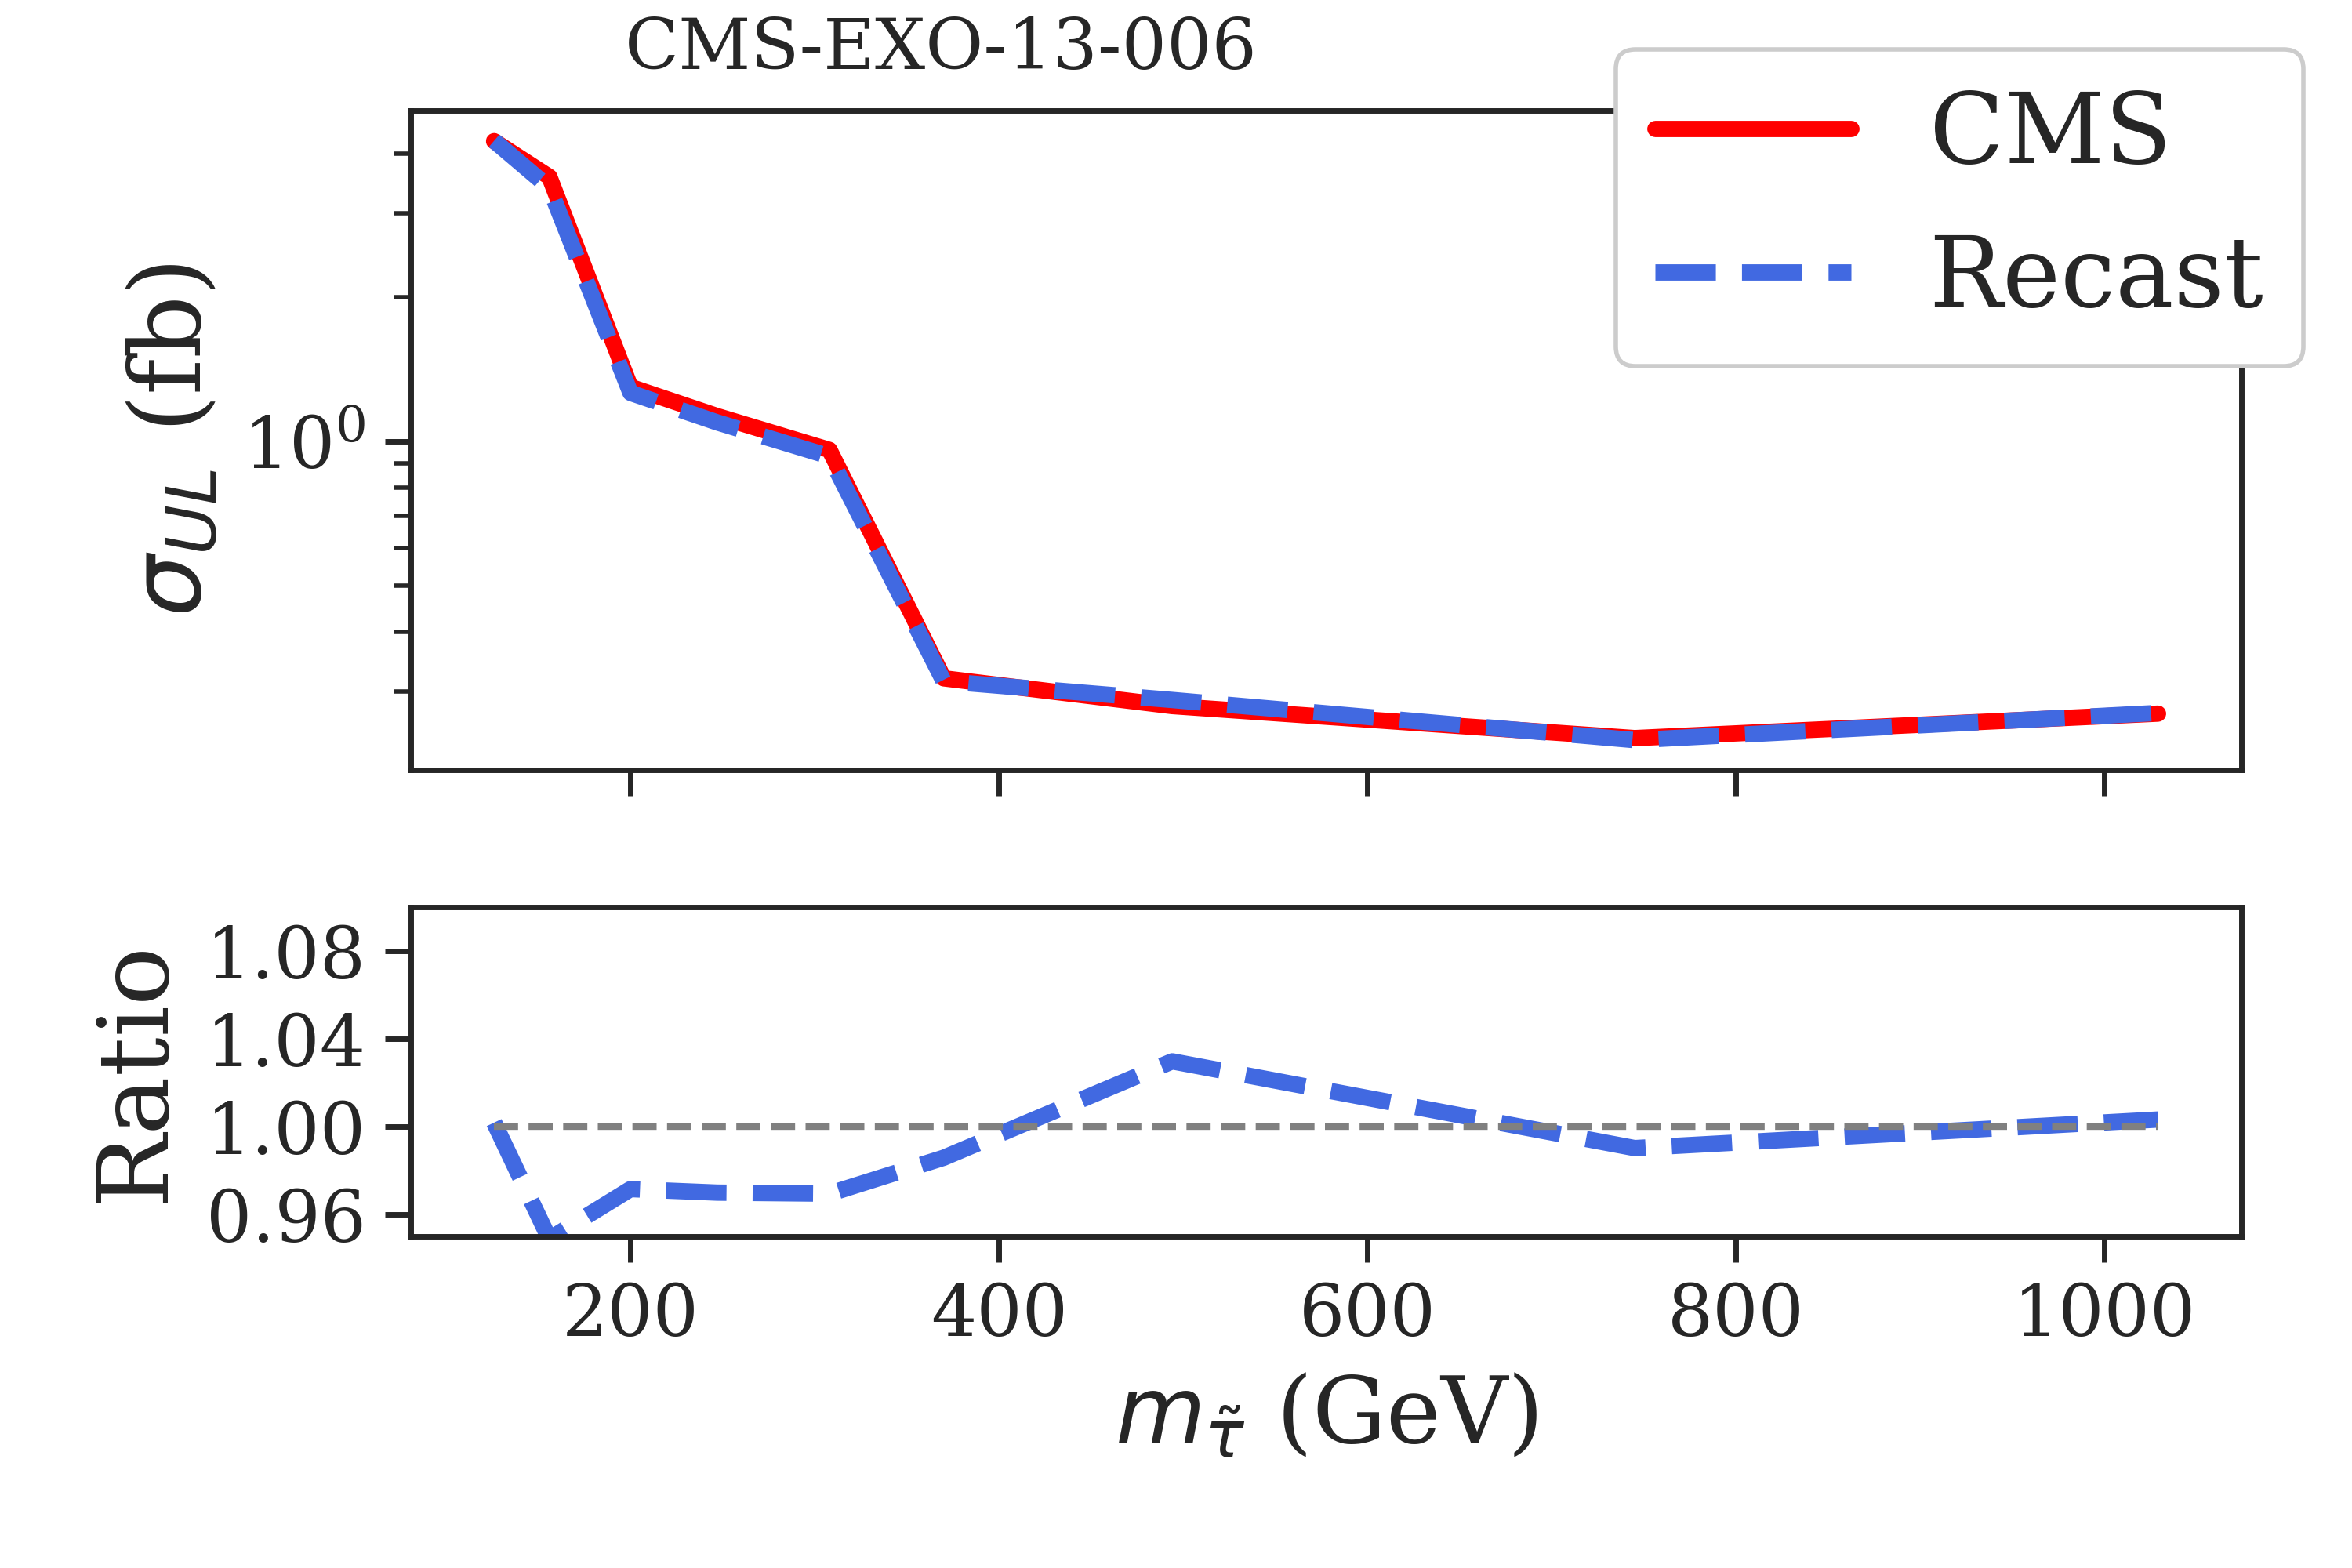
\includegraphics[clip, trim={0.1cm 0.4cm 0cm 0cm}, width=0.46\textwidth]{figures/ULratio_CMS-EXO-13-006_stau.png}}
\put(0.5,0.0){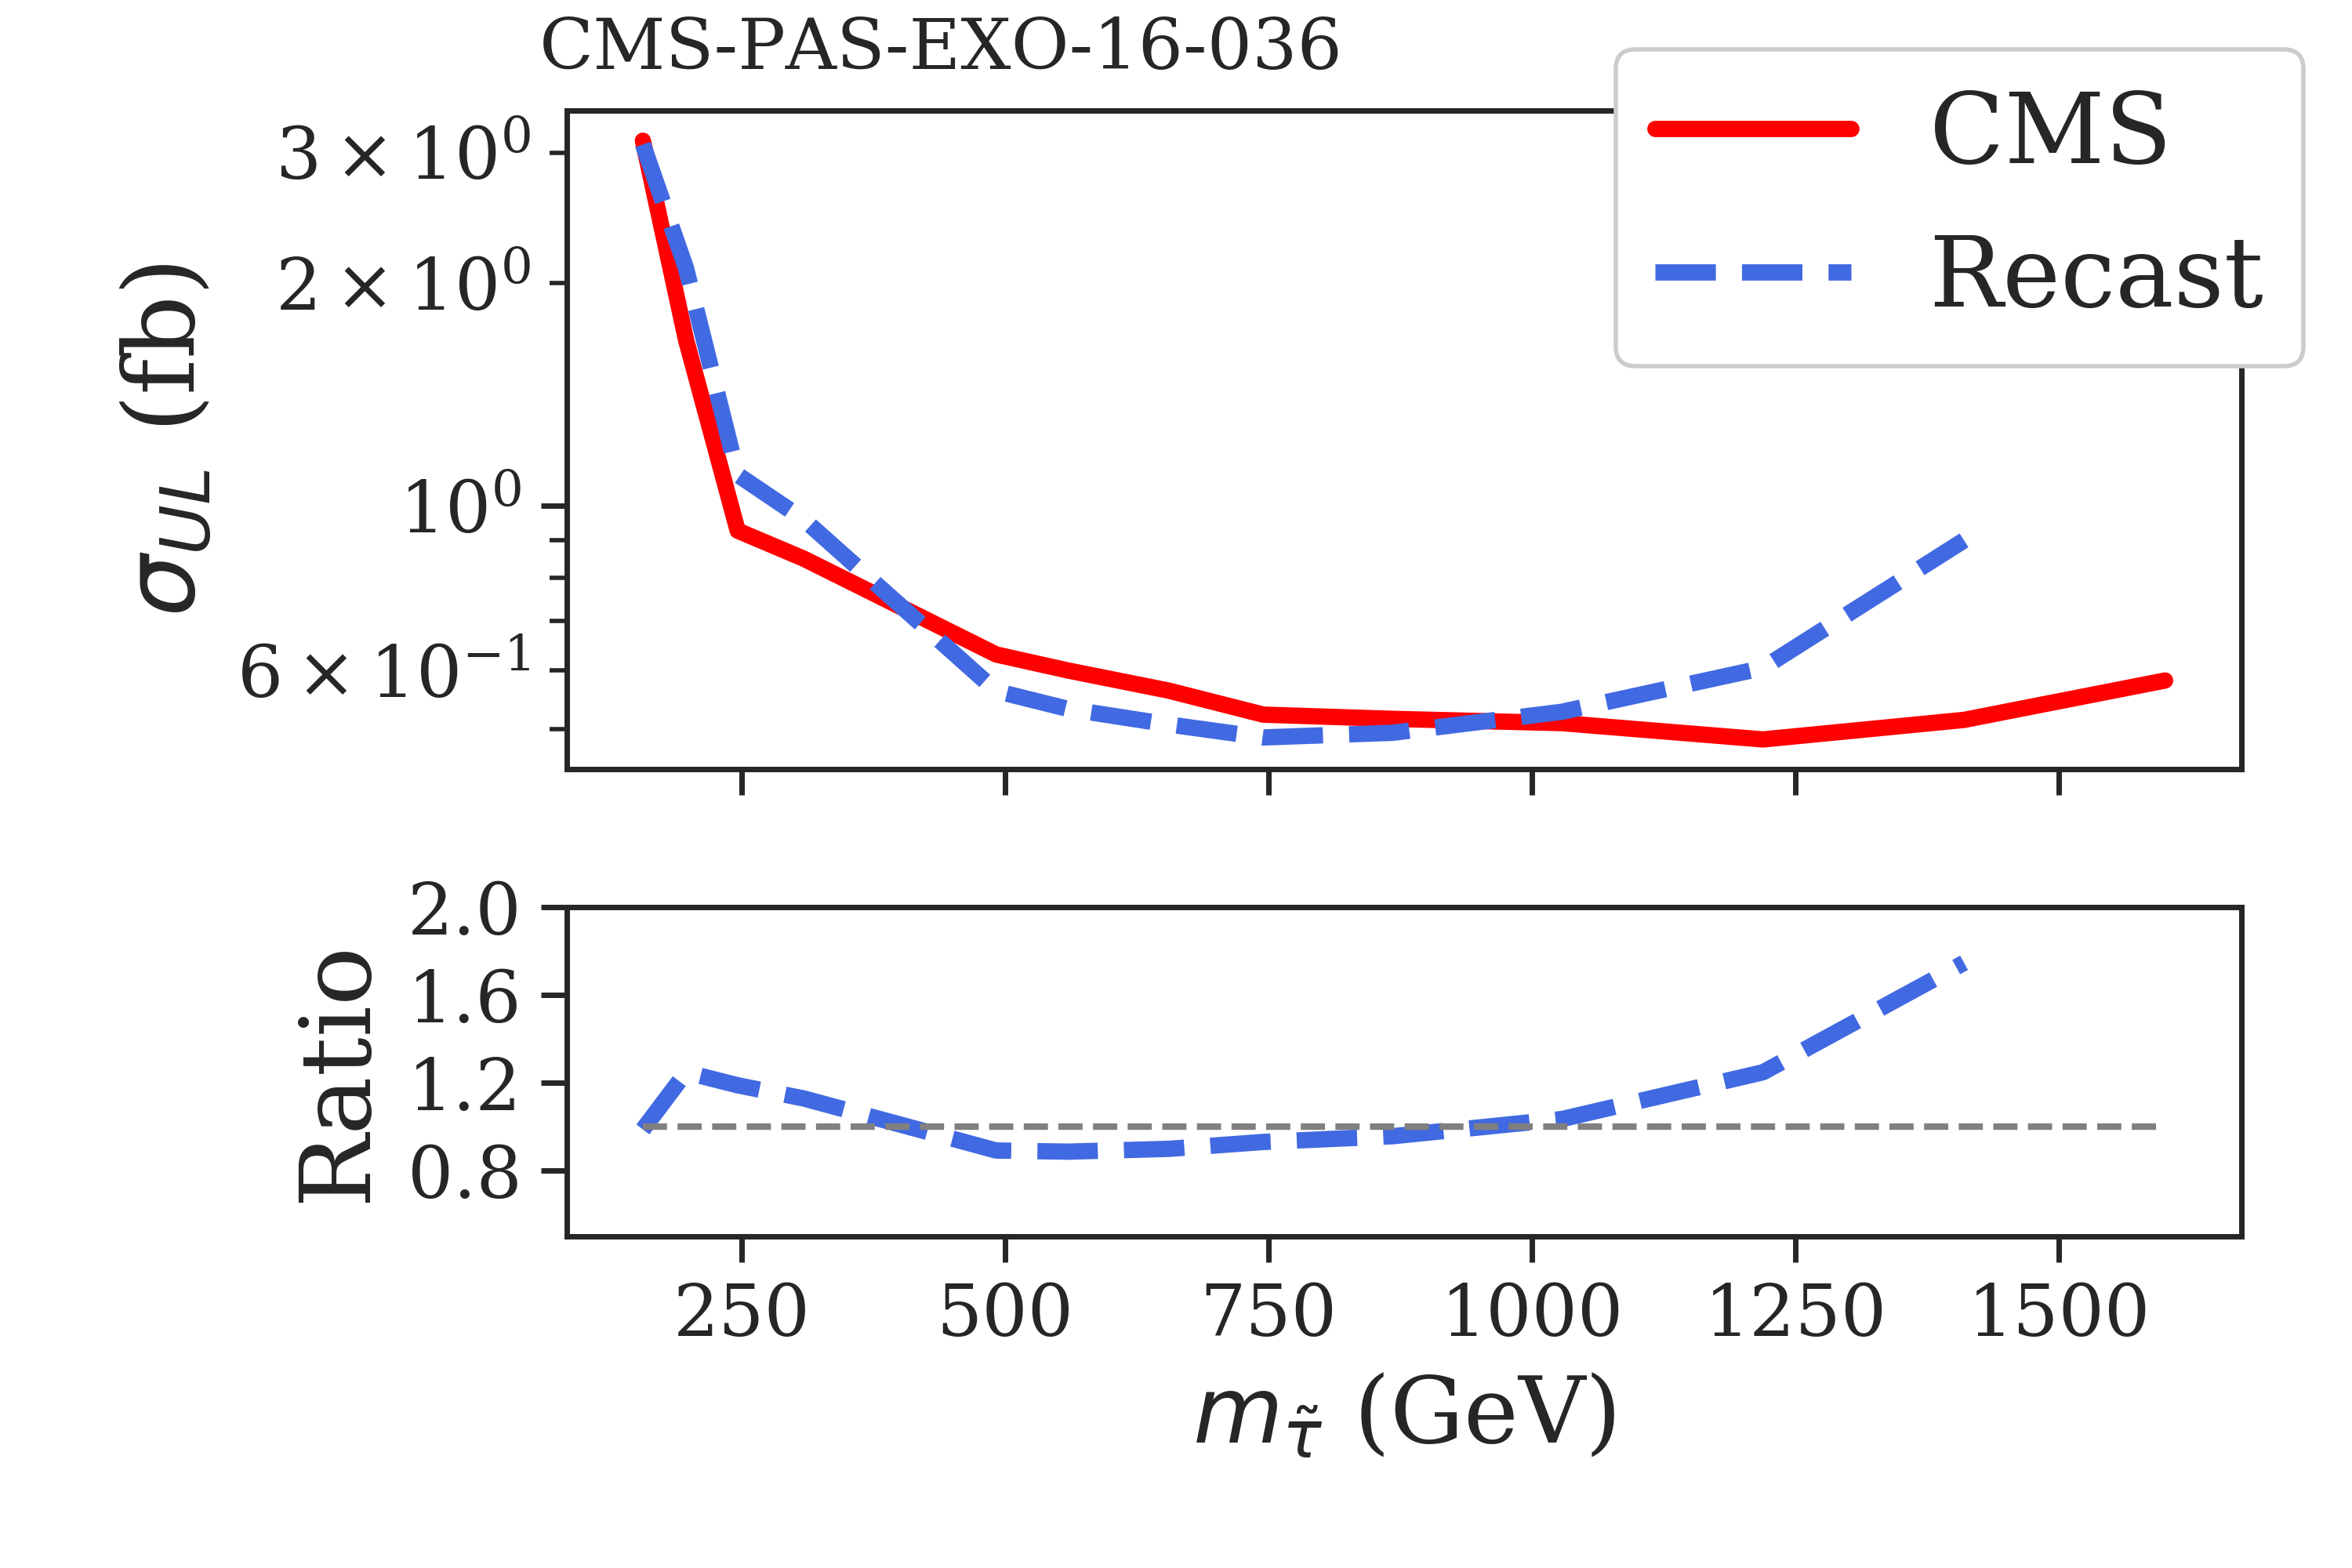
\includegraphics[clip, trim={0.1cm 0.4cm 0cm 0cm}, width=0.46\textwidth]{figures/ULratio_CMS-PAS-EXO-16-036_stau.png}}
\end{picture}
\caption{Validation of the 8\,TeV (left panel) and 13\,TeV (right panel) CMS analysis for direct production of staus.
The red and blue dashed curves show the respective cross-section upper limits from CMS and from our recast.
}
\label{fig:vali}
\end{figure*}
%                                      \         |
%                                        \       |
%                                          \     |
%=======================
In this appendix we detail the recasting of the 8 and 13\,TeV HSCP searches used in \smo. We first review the 
recasting for the 8\,TeV CMS HSCP analysis presented in~\cite{Khachatryan:2015lla}. The authors of~\cite{Khachatryan:2015lla} provide
signature efficiencies for the off- and online selection criteria, $P_\text{on}(\vec{k})$ and $P_\text{off}(\vec{k})$, respectively, as a function of the generator-level kinematics, $\vec{k}=(\eta,p_\text{T},\beta)$, of isolated\footnote{Details on the imposed isolation criteria can be found in~\cite{Khachatryan:2015lla,Heisig:2015yla}.} HSCP candidates.
The signal efficiency for a given parameter point can be computed from the generated events:
\begin{equation}
\label{eq:signaleff}
({\cal A}\epsilon) = \frac{1}{N}\sum_{i=1}^N {\cal P}^{\,i}_\text{event} 
\end{equation}
where the sum runs over all $N$ events and
\begin{equation}
\label{eq:pevent}
{\cal P}^{\,i}_\text{event} ={\cal P}^{\,i}_\text{on}\times {\cal P}^{\,i}_\text{off}
\end{equation}
with
\begin{equation}
\begin{split}
{\cal P}^{\,i}_\text{on/off} = &\;P_\text{on/off}(\vec{k}_1^i) + P_\text{on/off}(\vec{k}_2^i)\\
& - P_\text{on/off}(\vec{k}_1^i)\times P_\text{on/off}(\vec{k}_2^i)\,.
\end{split}
\end{equation}
For one HSCP candidate in an event the formula holds with $P_\text{on/off}(\vec{k}_2^i)=0$.


Using the efficiencies computed using \ref{eq:signaleff} for the direct pair production of staus and the observed and expected number of background events (along with its error) from Ref.\cite{Khachatryan:2015lla}
we obtain upper limits for the stau cross-section as a function of the stau mass. These can then be directly compared to the CMS values presented in Ref.\cite{Khachatryan:2015lla}. 
The left panel of figure~\ref{fig:vali} shows the CMS and our results for the cross-section upper limits as well as their ratio (lower frame). As we can see, the difference is always below 5\% and compatible with Monte Carlo errors. Hence we expect that recasting uncertainties for the efficiencies computed with the above method and included in the \smo\ database should
only be of a few percent.



For the respective 13\,TeV analysis~\cite{CMS-PAS-EXO-16-036}, however, such a recast has not yet been provided. Nonetheless, since the trigger and selection criteria of the 8 and 13\,TeV analyses are very similar, we 
expect that the signal efficiencies from the 8~TeV search do not
differ drastically from the 13~TeV ones.
The two analyses only differ in a slightly stronger cut on the ionization loss and time-of-flight, which effectively amounts
to a slightly stronger cut on the HSCP velocity in the latter analysis.\footnote{The effect of slightly stronger cut on $p_\text{T}$~\cite{CMS-PAS-EXO-16-036} is found to be negligible for masses of a few hundred GeV.}
Ref.~\cite{Brooijmans:2018xbu}
reported an attempt to model the 13\,TeV signature efficiencies by multiplying the 8\,TeV ones with
a velocity dependent correction function fitted in order to resemble the signal efficiencies reported in~\cite{CMS-PAS-EXO-16-036}.
On top of the slight reduction of the signature efficiencies for high velocities this study revealed a better performance of the CMS detector in the region of low velocities leading to larger signal efficiencies
for large HSCP masses. This latter feature could, however, not be described by a universal velocity dependent correction function for direct pair production and inclusive production. In order for a proper understanding of the differences between Runs 1 and 2, further information (which is not publicly available) is needed.
Therefore we choose to follow a conservative approach taking into account the reduction in the efficiency due to the slightly
stronger cuts on the velocity of the HSCP candidate. 
We model this by multiplying $P_\text{off}(\vec{k})$ with a correction function which is assumed to depend only on $\beta$:
\begin{equation}
f_{(a,b)}^\text{corr}(\beta) = \left(1+\E^{a (\beta-b)}\right)^{-1}\le1
\end{equation}
We determine the parameters $a,b$ in a 
global fit to the signal efficiencies for the pair production and inclusive production model reported in Ref.~\cite{CMS-PAS-EXO-16-036}. 
To this end we define the $\chi^2$ function:
\begin{equation}
\label{eq:chi2}
\chi^2 = \sum_m \frac{\left(({\cal A}\epsilon)^m_{(a,b)} - ({\cal A}\epsilon)^m_\text{CMS}\right)^2}{\sigma_{{\cal A}\epsilon}^2}\,,
\end{equation}
where $({\cal A}\epsilon)^m_{(a,b)}$ is the signal efficiency for a mass point $m$ of the considered model
using the signature efficiencies with the correction function $f_{(a,b)}^\text{corr}$ and $({\cal A}\epsilon)^m_\text{CMS}$ is the 
respective signal efficiency reported by CMS in Ref.~\cite{CMS-PAS-EXO-16-036}. The
characteristic size of the uncertainty, $\sigma_{\!{\cal A}\epsilon}$, is (arbitrarily) set to $0.02$, which roughly
reflects the precision of the recasting we aim at.
We minimize the $\chi^2$ using \textsc{Multinest}~\cite{Feroz:2008xx,Feroz:2013hea} 
%to explore the parameter space. The fit turns out to prefer a very sharp cut in $\beta$ resembling 
%an approximate Heaviside step function for which the value of 
%$a$ is not constrained beyond being larger than $150$. 
and obtain the best-fit parameters: $a\simeq 500 $ and $b=0.807$. This fit was obtained using all the 12 benchmark points (6 for direct stau production and 6 for inclusive production) considered in Ref.\cite{CMS-PAS-EXO-16-036} and for which 
signal efficiencies were reported.
However, we have verified that very similar results are obtained when using only a subset of the benchmark points.
Once again we compare the upper limits for the total stau direct production cross-section obtained using our recast procedure and the ones reported by CMS. The comparison is shown by the right panel of Fig.~\ref{fig:vali},
where see that, despite having a worse agreement than the 8~TeV results,
the 13~TeV upper limits are within 20\% while for large range of stau masses. Only for $m_{\tilde \tau} \gtrsim 1.2$~TeV the 
recasting significantly diverges from the official values. We point out, however, that the results are still conservative due to the above mentioned effects.



%
%
%%=======================
%%    \                                           |
%%      \                                         |
%%        \                                       |
%\begin{figure}[t]
%\centering
%\setlength{\unitlength}{1\textwidth}
%\begin{picture}(0.4,0.38)
%\put(0.0,0.0){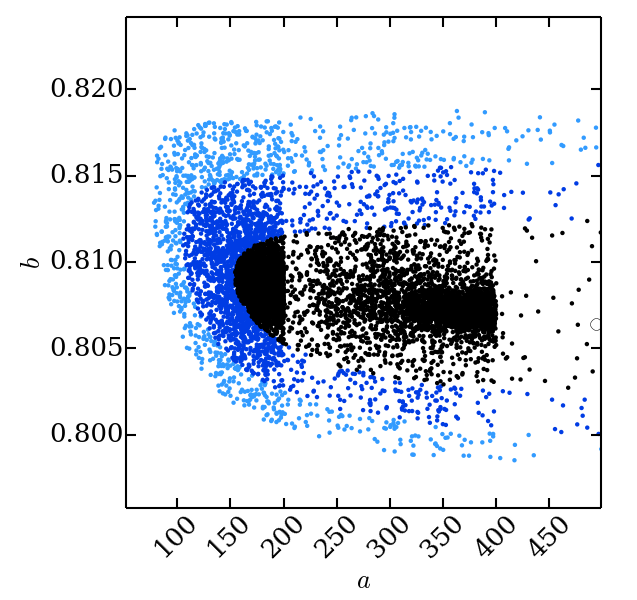
\includegraphics[clip, trim={0cm 0.1cm 0cm 0cm}, width=0.4\textwidth]{figures/fit13.png}}
%\end{picture}
%\caption{
%\com{I'm currently redoing the fit over the whole range just to obtain a set of points more smoothly distributed.}
%}
%\label{fig:}
%\end{figure}
%%                                      \         |
%%                                        \       |
%%                                          \     |
%%=======================
%


%===================================================================
\section{Finite lifetimes}\label{app:lifetime}
%===================================================================

%=======================
%    \                                           |
%      \                                         |
%        \                                       |
\begin{figure*}[h]
\centering
\setlength{\unitlength}{1\textwidth}
\begin{picture}(1,0.4)
\put(0.0,0.0){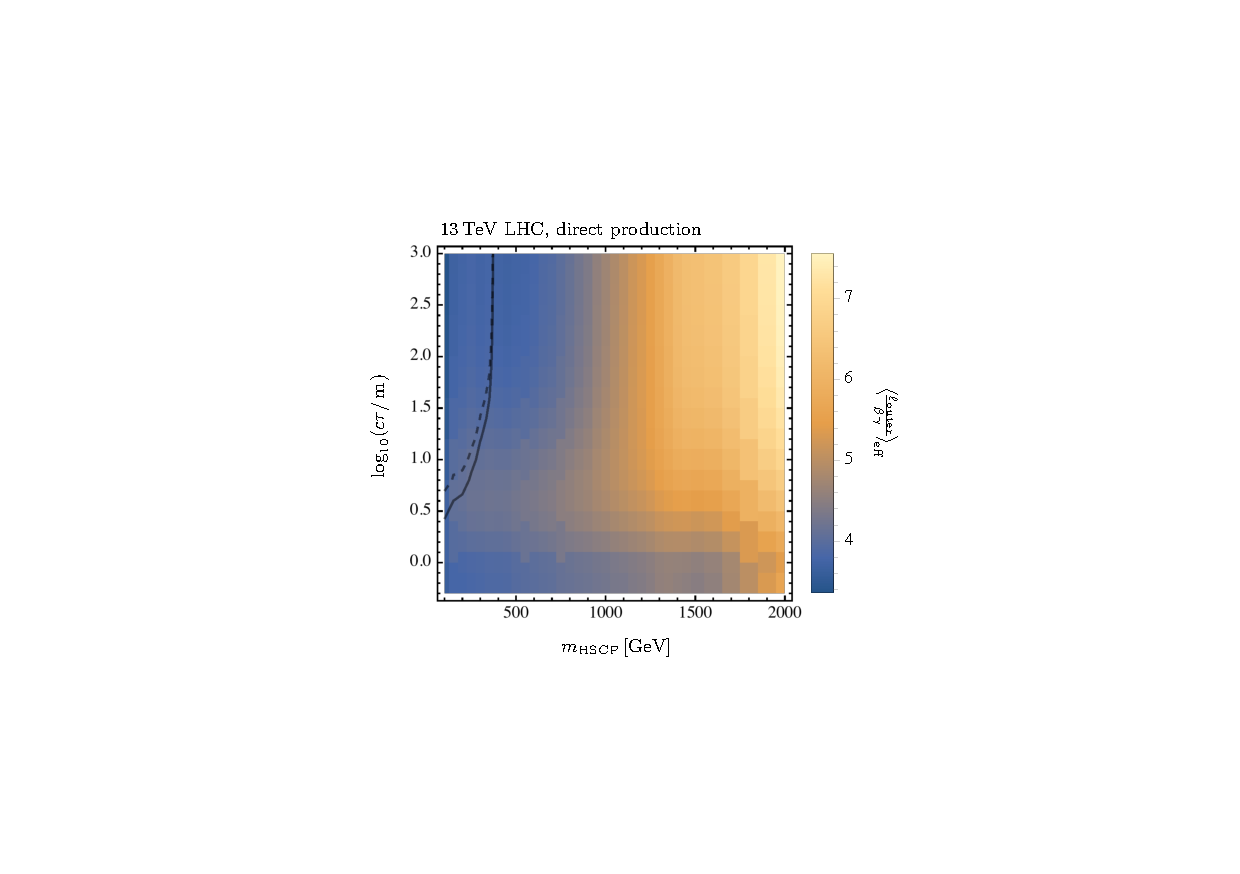
\includegraphics[clip, trim={6.15cm 3.5cm 5.5cm 3cm}, width=0.505\textwidth]{figures/plot_gammabeta_direct.pdf}}
\put(0.505,0.0){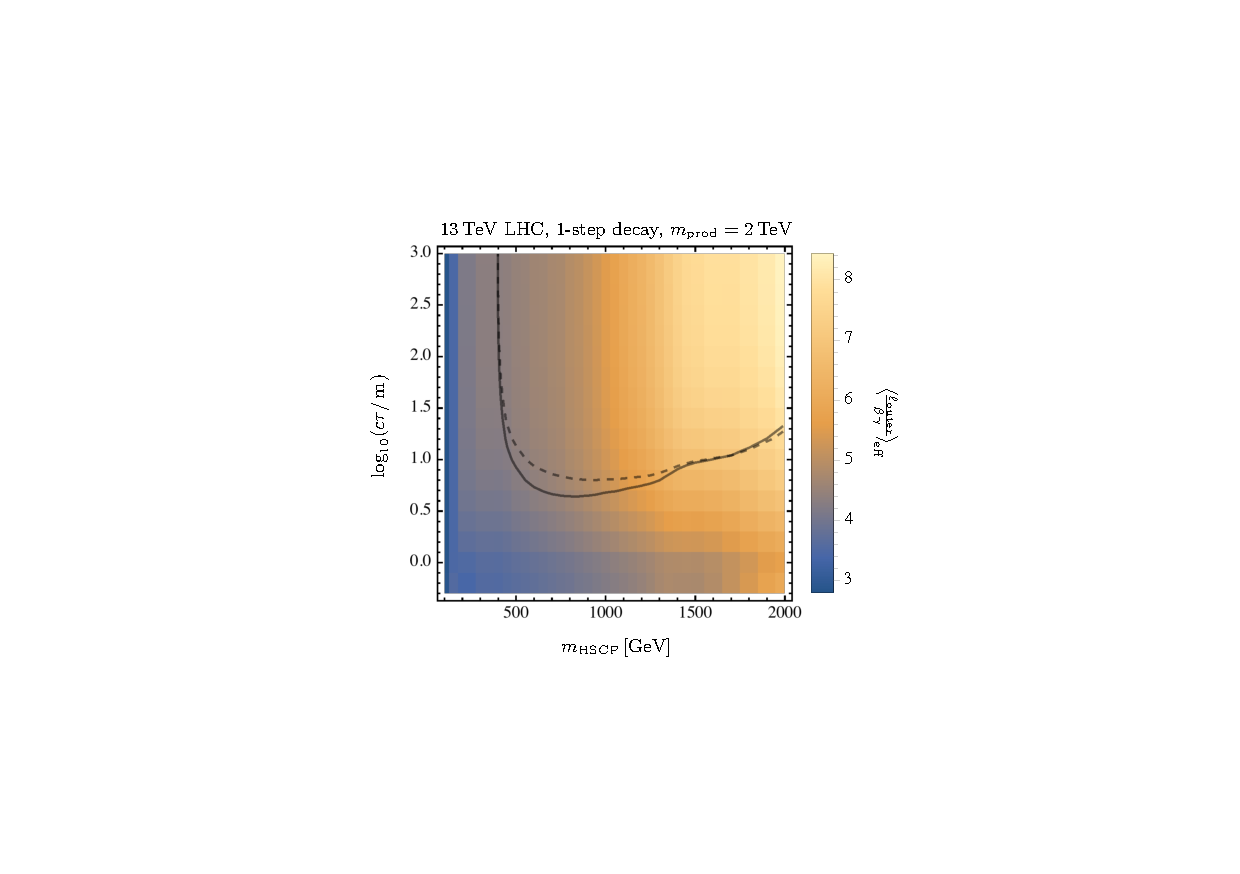
\includegraphics[clip, trim={6.15cm 3.5cm 5.5cm 3cm}, width=0.505\textwidth]{figures/plot_gammabeta_1step.pdf}}
\end{picture}
\caption{The effective characteristic travel length, $\langle\ell_\text{outer}/\gamma\beta\rangle_\text{eff}$ (see text for details) in the parameter plane spanned by the HSCP mass, $m_\text{HSCP}$, and its proper decay length, $c\tau$ for direct production (left panel) and for the 1-step decay topology where we choose $m_\text{prod}=2\,$TeV for the mass of the produced mother particle (right panel). The solid and dashed curves denote the 95\% CL exclusion for the event-based computation of $\ell/\gamma\beta$ and for the approximation choosing $\langle\ell_\text{outer}/\gamma\beta\rangle_\text{eff}=7\,$m (see text for details). For the direct production we choose the cross-section Drell-Yan stau pair production, while the cross-section for 1-step decay corresponds to (degenerate) squark production with $m_{\tilde q}=m_{\tilde g}$.
}
\label{fig:leff}
\end{figure*}
%                                      \         |
%                                        \       |
%                                          \     |
%=======================

Although the HSCP searches considered here are aimed for detector-stable particles
they can also constrain models with intermediate decay length of the order of the detector size
where only a certain fraction of particles decay after traversing the entire sensitive detector. In this case the fraction of long-lived particles, ${\cal F}_\mathrm{long}$, may be significantly smaller than one and the resulting signal efficiency becomes sensitive to value chosen for $L_{eff} \equiv \langle\ell_\text{outer}/\gamma\beta\rangle_\text{eff}$ (see eq.\ref{eq:Flong}).
Here we discuss in detail what are the expected values for $L_{eff}$ and justify our choice, $L_{eff}  = 7$~m, used in the results presented in Sec.\ref{sec:physapp} and implemented in \smo~1.2. 


The precise value of ${\cal F}_\mathrm{long}$ (and hence $L_{eff}$) 
actually depends on the input model and experimental analysis and
requires a full Monte Carlo simulation for each model point in order to determine the boost distribution of the HSCP particles. However, since \smo\ aims for a fast (although approximate)
computation of LHC constraints for a large variety of BSM models, our
goal is to determine an average value for $L_{eff}$ which can approximately reproduce the correct value of ${\cal F}_\mathrm{long}$ obtained from a full simulation.
Before we can justify this approximation, we must first discuss how to obtain  ${\cal F}_\mathrm{long}$ from the full simulation for a given input model. 


We first define the probability for a (metastable) particle with momentum $\vec{k}$ to decay outside the detector in a given event:
\begin{equation}
\label{eq:flongevt}
F_\text{long}(\vec{k}) = \exp\left(-\frac{\ell_\text{outer}(|\eta|)}{\gamma \beta }\frac{1}{c\tau}\right)\,.
\end{equation}
Here $\gamma = (1-\beta^2)^{-1/2}$ and $\ell_\text{outer}(|\eta|)$ is the travel length
through the CMS detector which we approximate by considering a cylindrical volume with radius of 7.4\,m and length of 10.8\,m.
Using now the off- and online efficiencies ($P_{\text{on}}$ and $P_{\text{off}}$) discussed in \ref{app:rec13}, we can
extend the signal efficiency calculation from
eq.~\eqref{eq:signaleff} to the case of finite lifetimes using:
\begin{equation}
\begin{split}
\label{eq:Pevfull}
{\cal P}^{\,i}_\text{event} = &\;
F_\mathrm{long}(\vec{k}_1^i)  P_{\text{on}}(\vec{k}_1^i) P_{\text{off}}(\vec{k}_1^i) \big(1- F_\mathrm{long}(\vec{k}_2^i)\big)\\
&\!\!\!+F_\mathrm{long}(\vec{k}_2^i)  P_{\text{on}}(\vec{k}_2^i) P_{\text{off}}(\vec{k}_2^i) \big(1- F_\mathrm{long}(\vec{k}_1^i)\big)\\
&\!\!\!+ F_\mathrm{long}(\vec{k}_1^i) F_\mathrm{long}(\vec{k}_2^i) {\cal P}^{\,i}_\text{on} {\cal P}^{\,i}_\text{off},
\end{split}
\end{equation}
where $F_\text{long}(\vec{k}_j^i)$ is the decay probability from eq.\ref{eq:flongevt} for the $j$-th particle in the $i$-th event.



Using eqs.\ref{eq:Pevfull} and \ref{eq:signaleff} we can then compute the total signal efficiency for a given input model taking into account the correct finite lifetime suppression factor. This factor can then be compared to the efficiency computed with \smo\ using ${\cal F}_\mathrm{long}$
to extract the precise value for $L_{eff}$ given a specific input model.
In Figure~\ref{fig:leff} we consider the direct production of staus (left panel) and direct production of squarks and gluinos followed by a 1-step decay to staus at the 13~TeV LHC.
In both models we vary the stau mass and lifetime, with $m_{\tilde g} = m_{\tilde q} = 2$~TeV for the second model.
The color of each point in the plane
shows the correct value for $L_{eff} = \langle\ell_\text{outer}/\gamma\beta\rangle_\text{eff}$ 
which should be used in \smo\ in order for the \smo\ signal efficiencies to exactly match the full simulation values.
As we can see, $L_{eff}$ does not vary significantly, spanning values within the interval $\sim$4-8~m. Therefore, in order to remain conservative 
and avoid (significantly) underestimating the signal efficiency we choose $L_{eff} = 7~m$ (or $l_\text{outer} = 10$~m and $\gamma\beta = 1.3$). 
Using this choice we show in Fig.~\ref{fig:leff} the corresponding exclusion curves obtained with \smo\ as dashed lines. We also display the corresponding curves obtained using the full simulation. 
Although the \smo\ curves are conservative, we see that they agree quite well with the full simulation in most of the parameter space. We therefore concluded that using a fixed $L_{eff} = 7$~m value is a valid approximation.


%\com{JH: I'm thinking if it's a good idea to introduce the $f$ (event based quantity) 
%to distinguish it from $\mathcal{F}$ which is some kind of averaged weight for 
%the respective parameter point. For $\mathcal{F}$ a formula like
%\begin{equation}
%\mathcal{F}_\text{prompt} = 1-\exp\left(-\frac{\ell_\text{inner}}{\gamma \beta} \frac{1}{c\tau}\right)
%\end{equation}
%is strictly speaking not properly defined (what is $\beta$?). So, it's just an ansatz after all. While for
%$f$ the formula is exact... I'm thinking what's the most efficient way to properly introduce it while not
%lengthen the discussion too much.}








%
%
%Describe decomposition and review the treatment regarding the probabilities ${\cal F}_\mathrm{long}/{\cal F}_\mathrm{prompt}$~\cite{Heisig:2015yla}. Discuss
%conservative estimate for $\gamma\beta$, show plot where proper treatment is compared
%to conservative choice. Mention~\cite{Brooijmans:2018xbu,Garny:2017rxs}.
%
%Formula used for ``proper treatment'': \com{here we could use the f}
%\begin{equation}
%\begin{split}
%P^{\,i}_\text{tot} = &\;
%{\cal F}_\mathrm{long}(\vec{k}_1^i)  P_{\text{on}}(\vec{k}_1^i) P_{\text{off}}(\vec{k}_1^i) \big(1- {\cal F}_\mathrm{long}(\vec{k}_2^i)\big)\\
%&\!+{\cal F}_\mathrm{long}(\vec{k}_2^i)  P_{\text{on}}(\vec{k}_2^i) P_{\text{off}}(\vec{k}_2^i) \big(1- {\cal F}_\mathrm{long}(\vec{k}_1^i)\big)\\
%&\!+ {\cal F}_\mathrm{long}(\vec{k}_1^i) {\cal F}_\mathrm{long}(\vec{k}_2^i) P^{\,i,(2)}_\text{on} P^{\,i,(2)}_\text{off}\,,
%\end{split}
%\end{equation}
%where 
%\begin{equation}
%\begin{split}
%P^{\,i,(2)}_\text{on/off} = &\;P_\text{on/off}(\vec{k}_1^i) + P_\text{on/off}(\vec{k}_2^i)\\
%& - P_\text{on/off}(\vec{k}_1^i)\times P_\text{on/off}(\vec{k}_2^i)\,.
%\end{split}
%\end{equation}

\end{appendix}
%%%%%%%%%%%


%\addcontentsline{toc}{section}{References}
%\bibliographystyle{utphys.bst}
%\bibliography{SModelS_HSCP_ref}

\end{document}

